\chapter{}
\label{appendix}

\section{Kinematics of the CBFs in the Middle/Outer Corona}
\label{ch2_append}
Here I present the extended measurements of the 26 EUV waves in the SOHO/LASCO FOV, up to \almost30 \rsun, and fitted with two CME kinematics models by \citet{gallagher_2003} and \citet{byrne_2013}. Overall, the Gallagher fitting model accommodated both AIA and LASCO measurements very well and proved the model's proficiency in capturing the early stages of the solar event, particularly in the lower corona.

\begin{figure}[!htp]
	\centering
	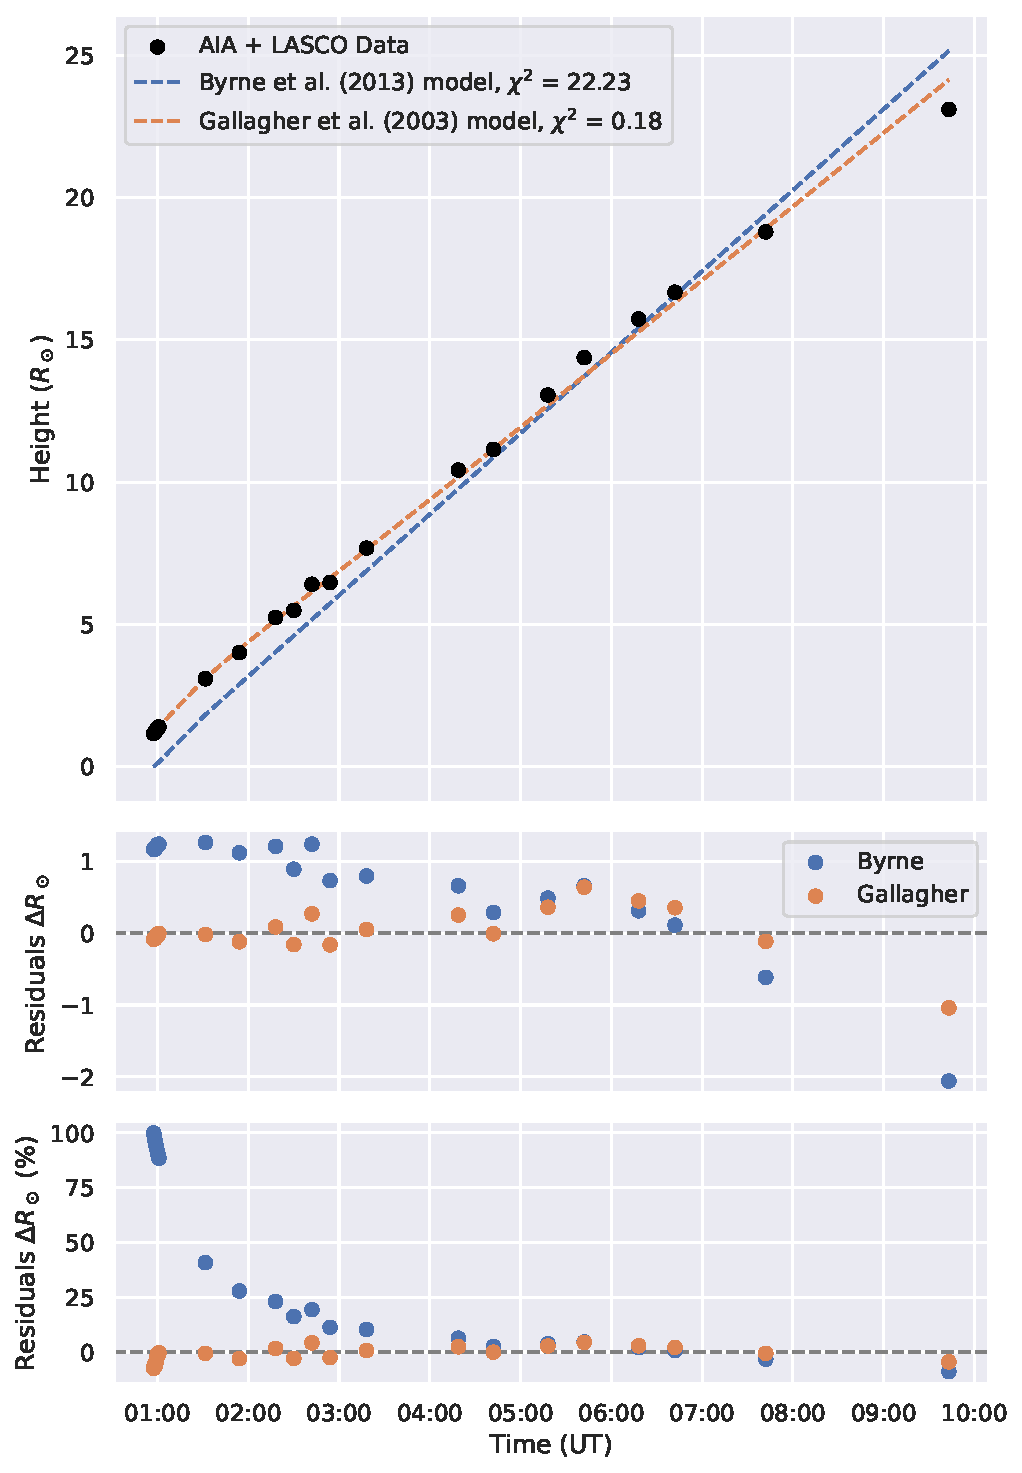
\includegraphics[width=0.8\hsize]{chapter2/figs/appendix/height_profile_residuals_aia_lasco_100612_01.pdf}
	\caption{Top panel: Height-time profile on June 12, 2010, using AIA and LASCO data, fitted with two CME kinematics models. Middle panel: Fitting vs. real observation difference. Bottom panel: Relative residuals in \%.}
\end{figure}

\begin{figure}[!htp]
	\centering
	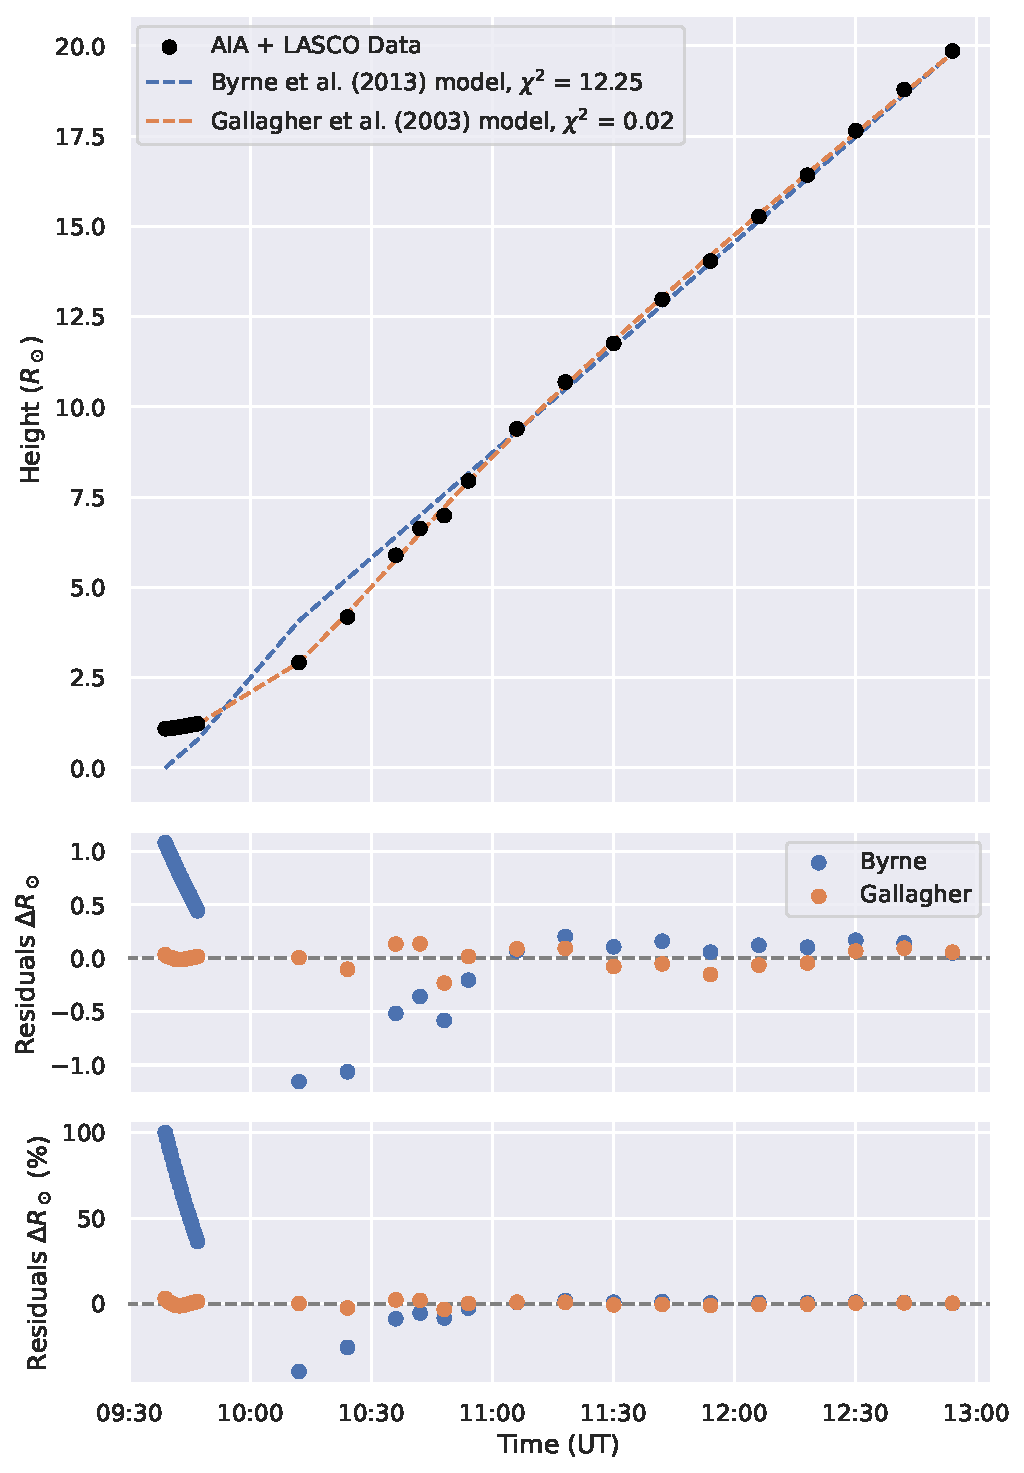
\includegraphics[width=0.8\hsize]{chapter2/figs/appendix/height_profile_residuals_aia_lasco_100814_01.pdf}
	\caption{Same for the event on August 14, 2010.}
\end{figure}

\begin{figure}[!htp]
	\centering
	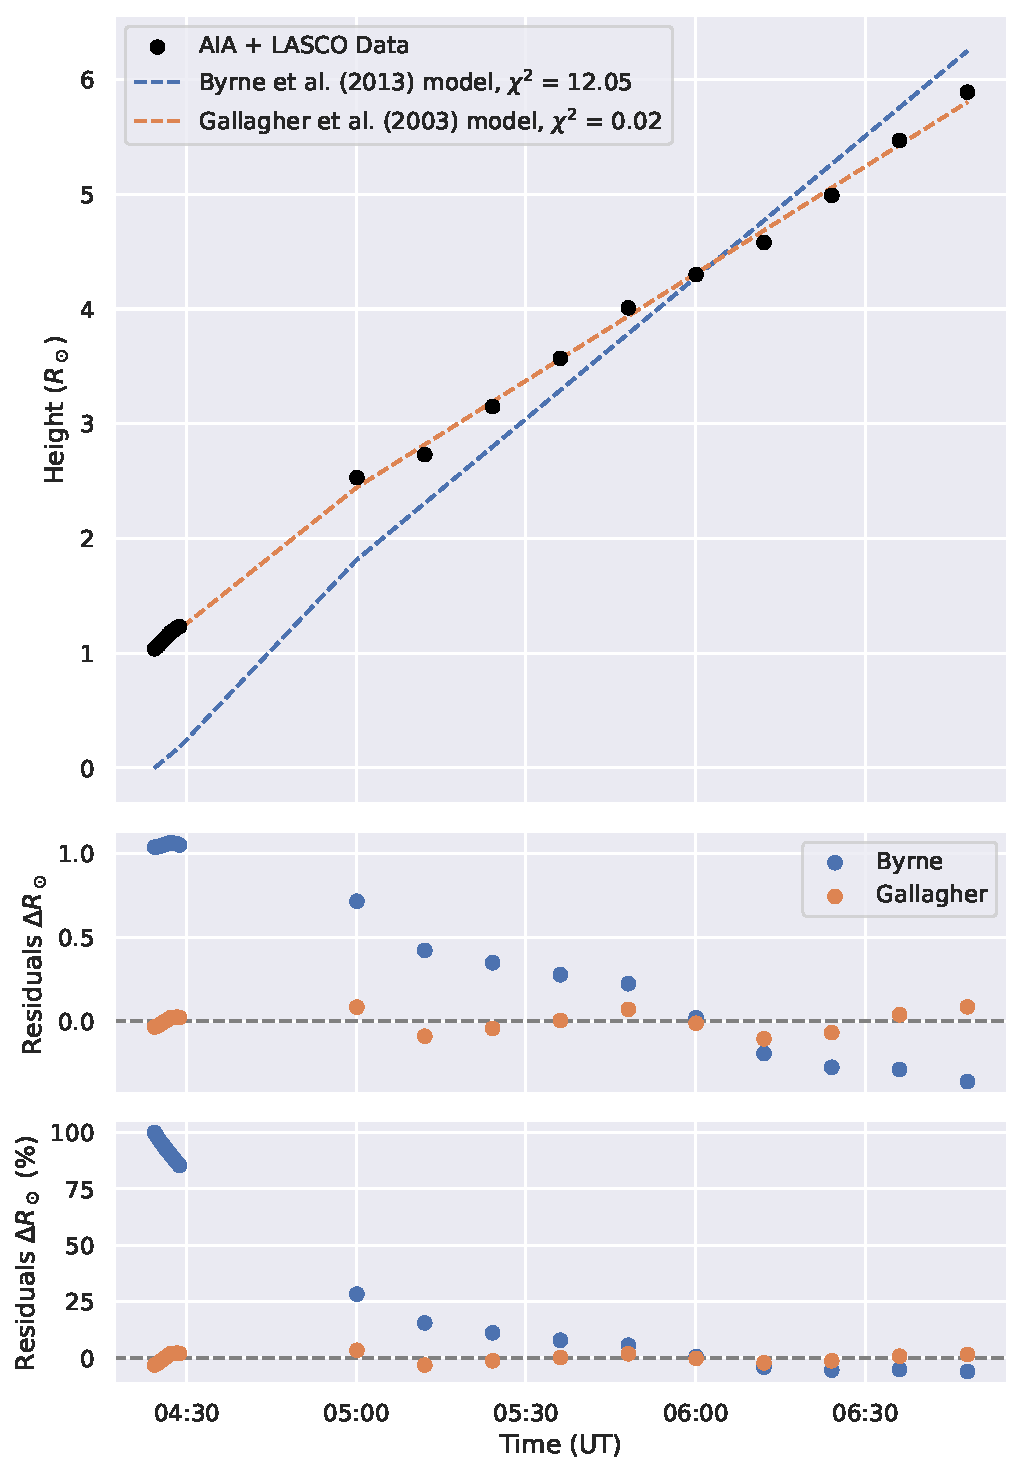
\includegraphics[width=0.8\hsize]{chapter2/figs/appendix/height_profile_residuals_aia_lasco_101231_01.pdf}
	\caption{Same for the event on December 31, 2010.}
\end{figure}

\begin{figure}[!htp]
	\centering
	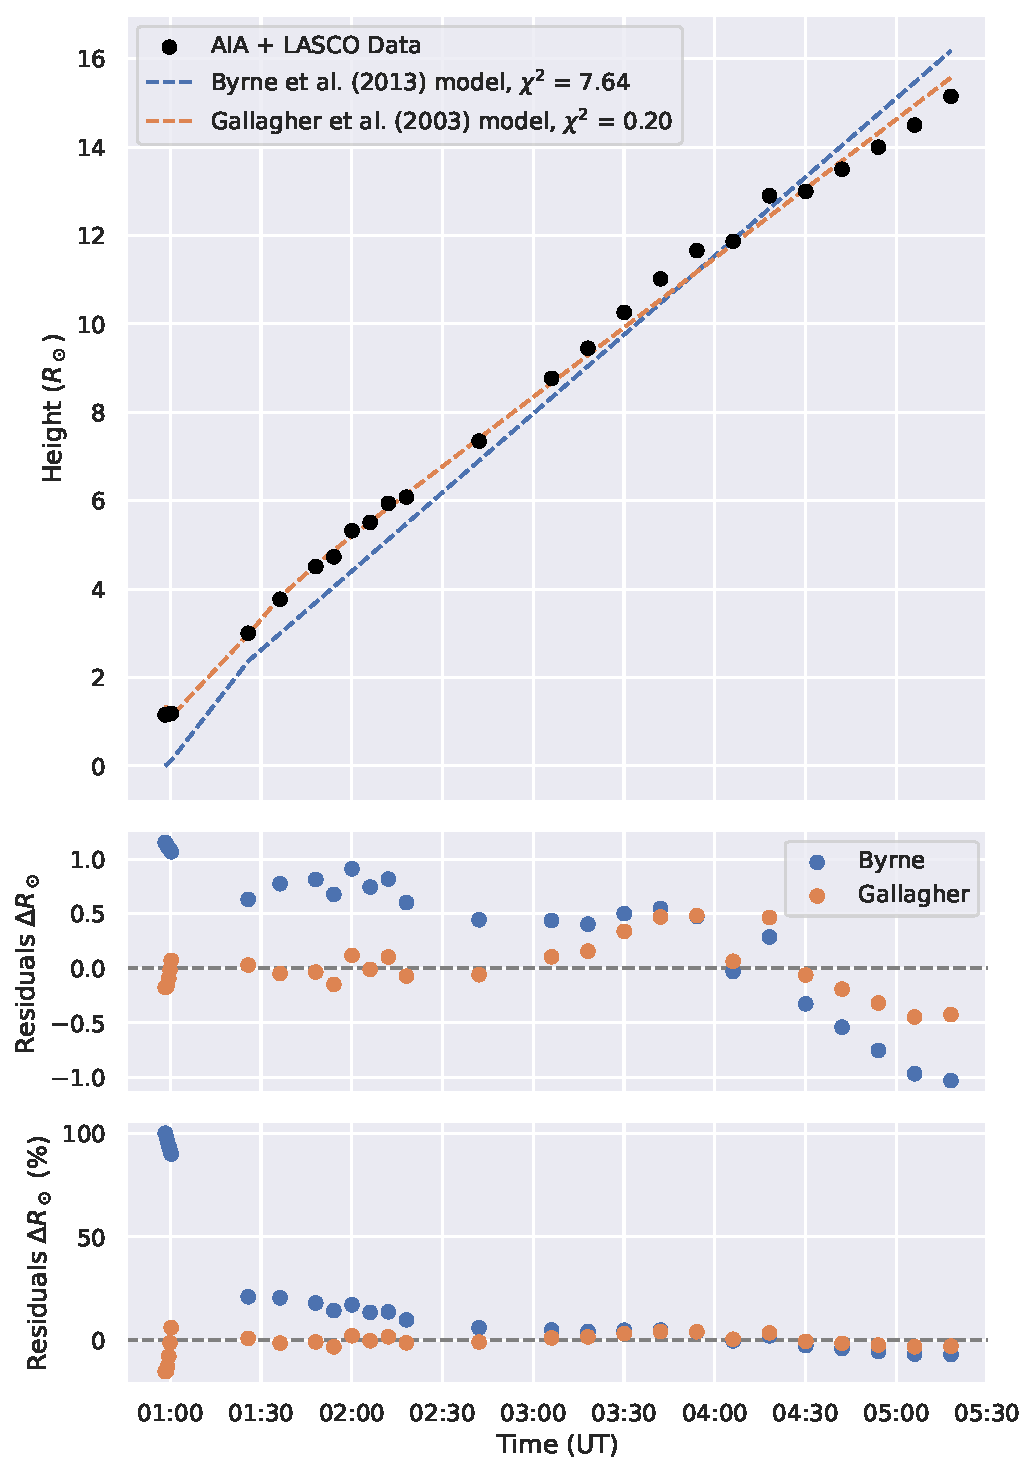
\includegraphics[width=0.8\hsize]{chapter2/figs/appendix/height_profile_residuals_aia_lasco_110128_01.pdf}
	\caption{Same for the event on January 28, 2011.}
\end{figure}

\begin{figure}[!htp]
	\centering
	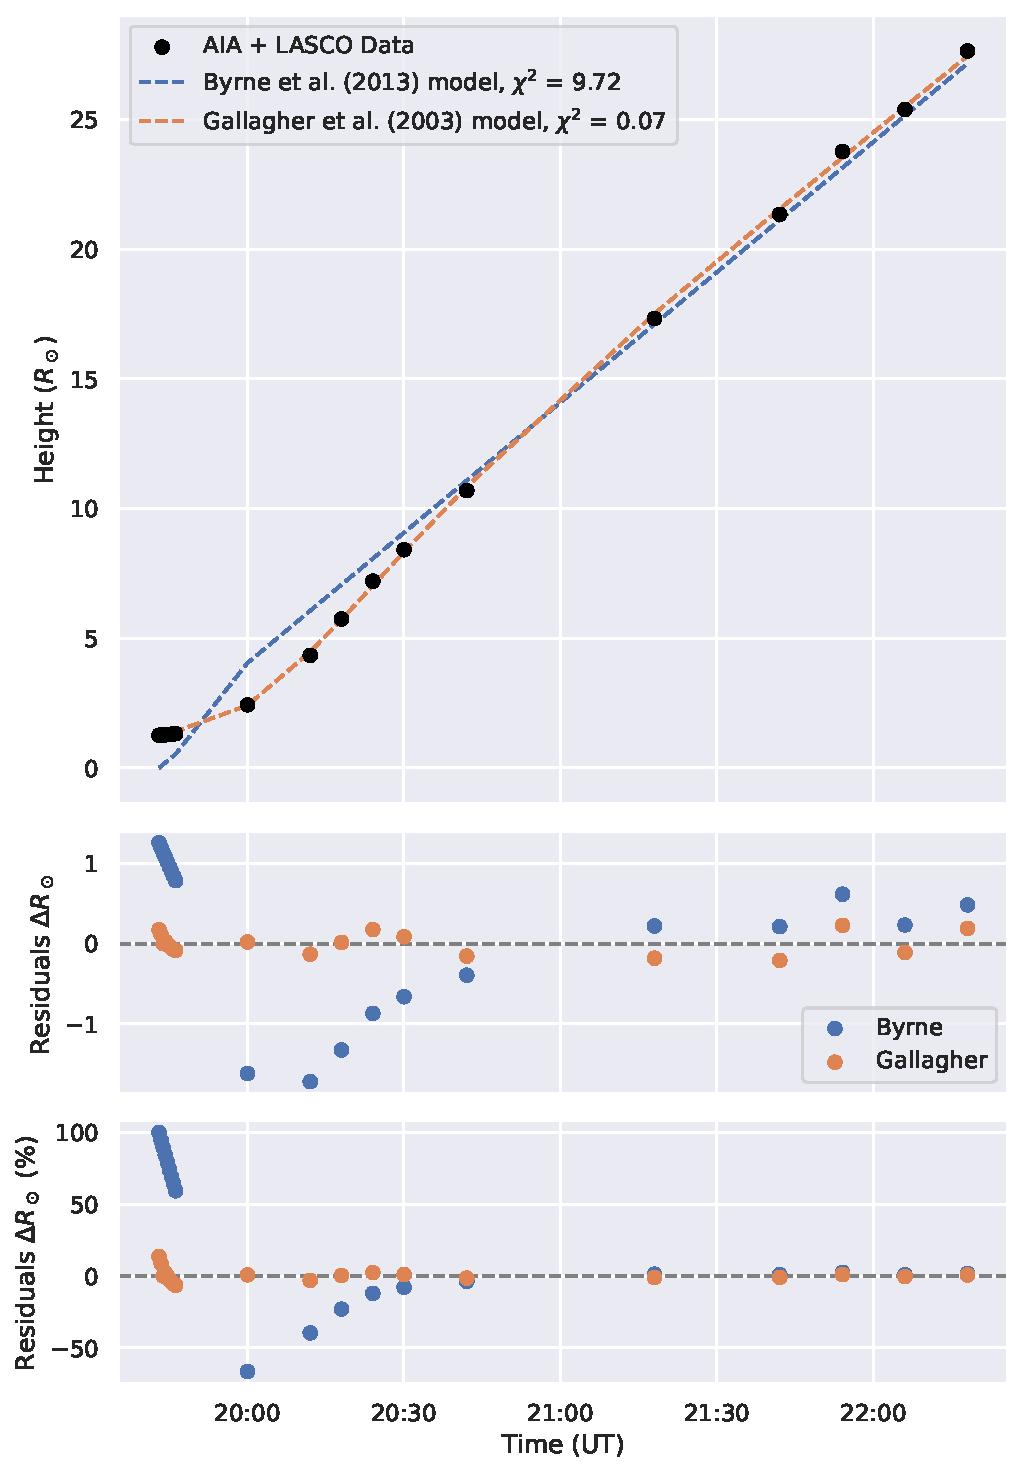
\includegraphics[width=0.8\hsize]{chapter2/figs/appendix/height_profile_residuals_aia_lasco_110307_02.pdf}
	\caption{Same for the event on March 7, 2011.}
\end{figure}

\begin{figure}[!htp]
	\centering
	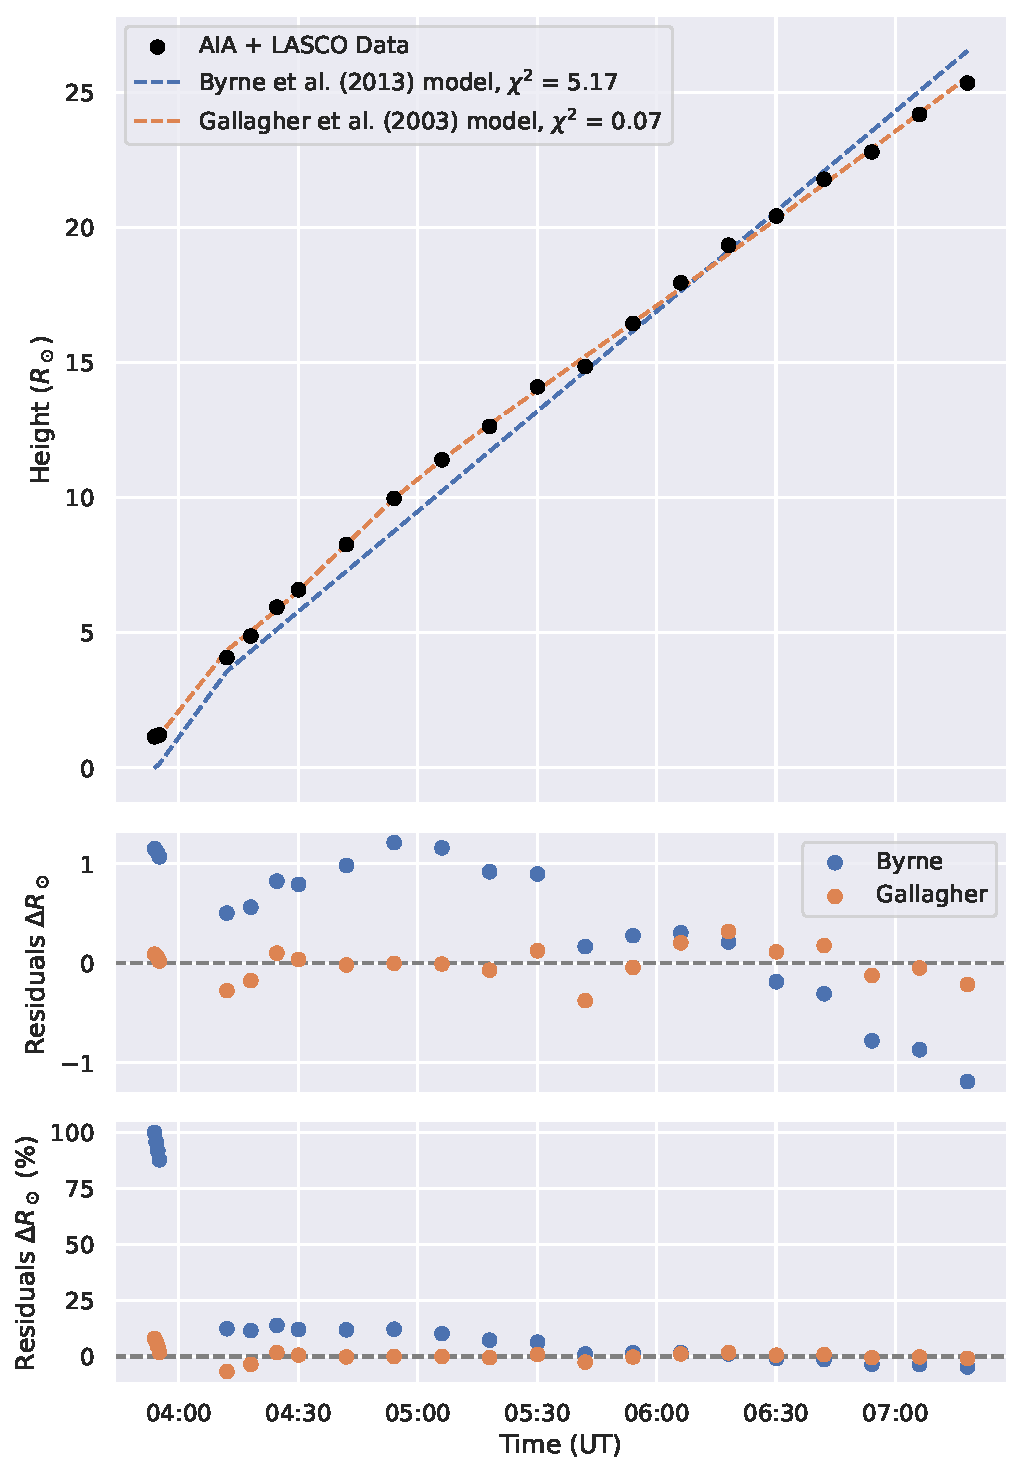
\includegraphics[width=0.8\hsize]{chapter2/figs/appendix/height_profile_residuals_aia_lasco_110804_01.pdf}
	\caption{Same for the event on August 4, 2011.}
\end{figure}

\begin{figure}[!htp]
	\centering
	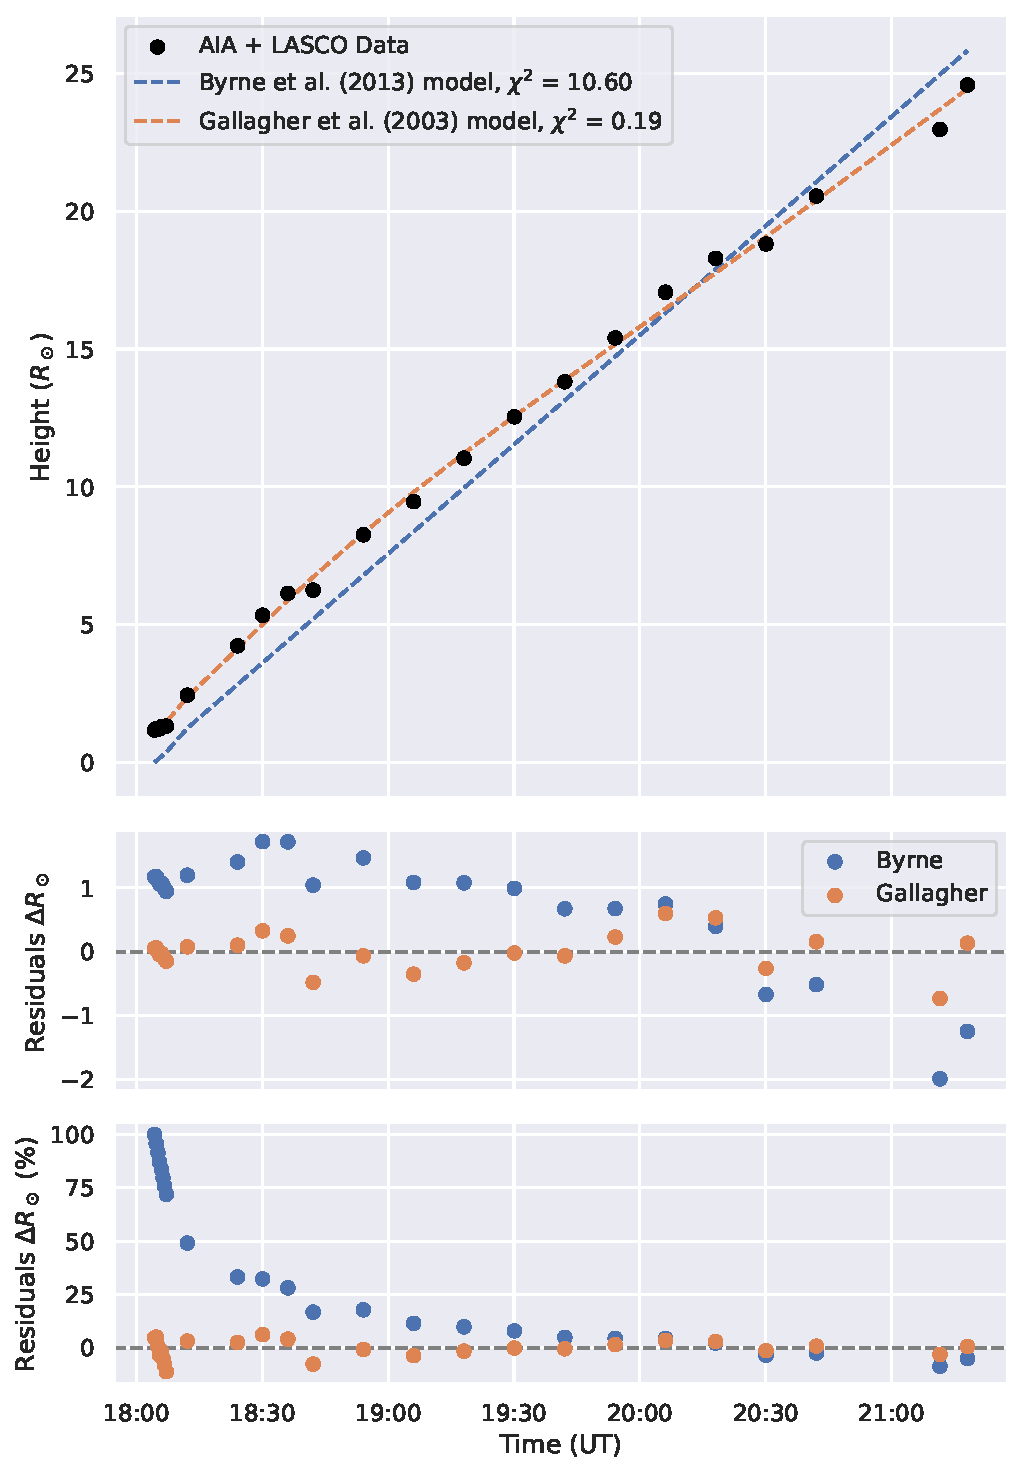
\includegraphics[width=0.8\hsize]{chapter2/figs/appendix/height_profile_residuals_aia_lasco_110808_01.pdf}
	\caption{Same for the event on August 8, 2011.}
\end{figure}

\begin{figure}[!htp]
	\centering
	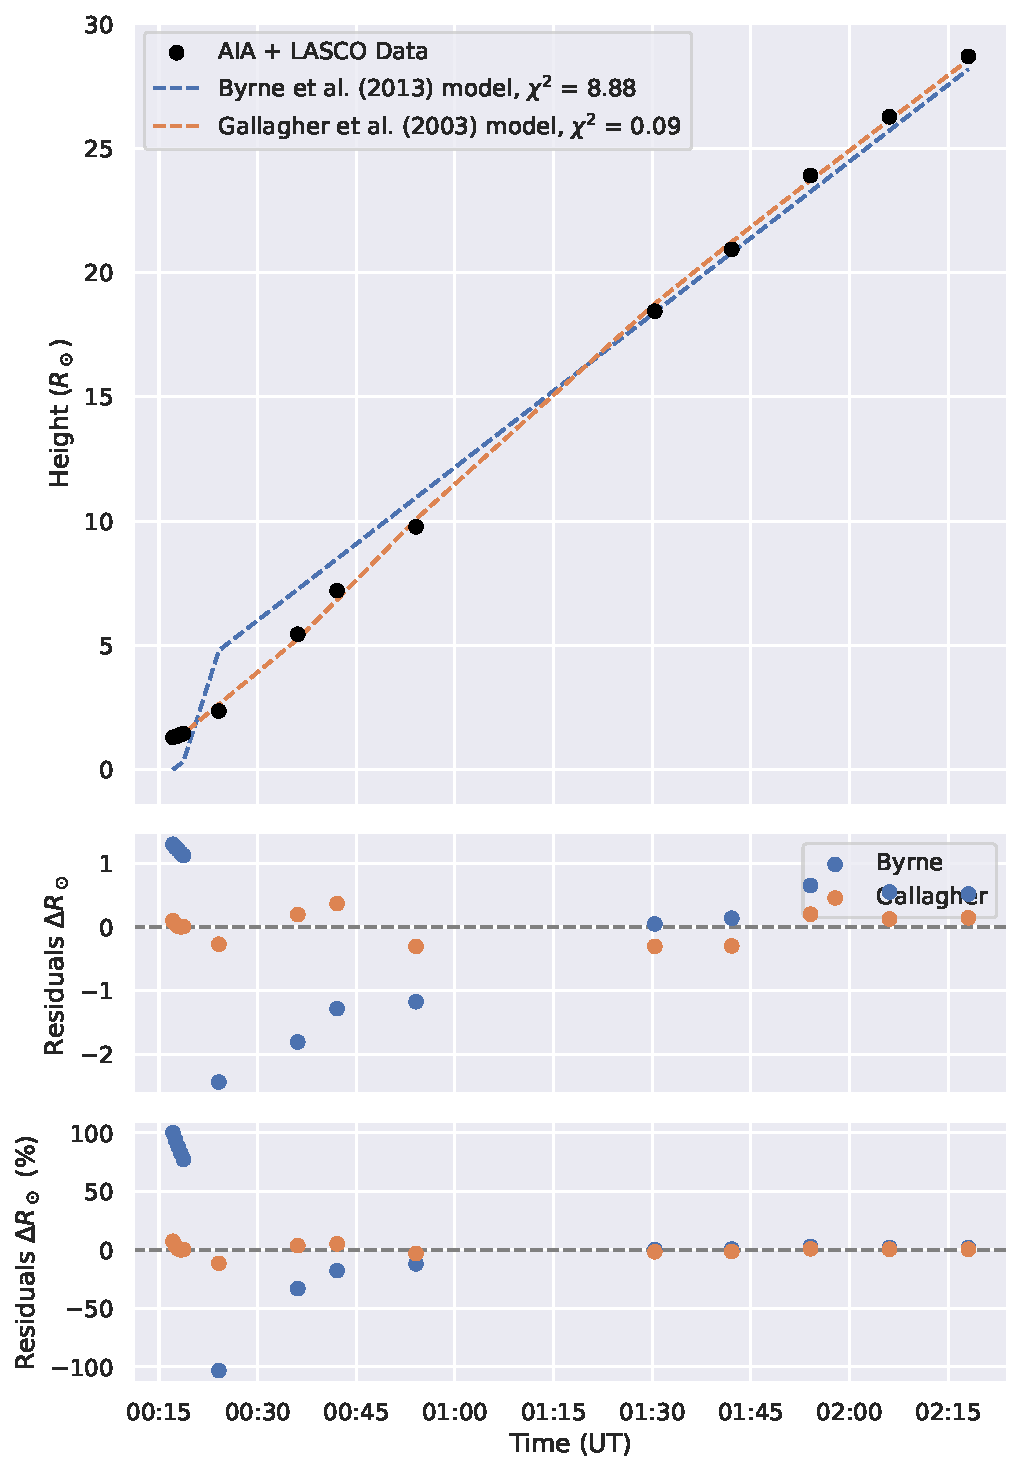
\includegraphics[width=0.8\hsize]{chapter2/figs/appendix/height_profile_residuals_aia_lasco_120307_01.pdf}
	\caption{Same for the event on March 7, 2012.}
\end{figure}

\begin{figure}[!htp]
	\centering
	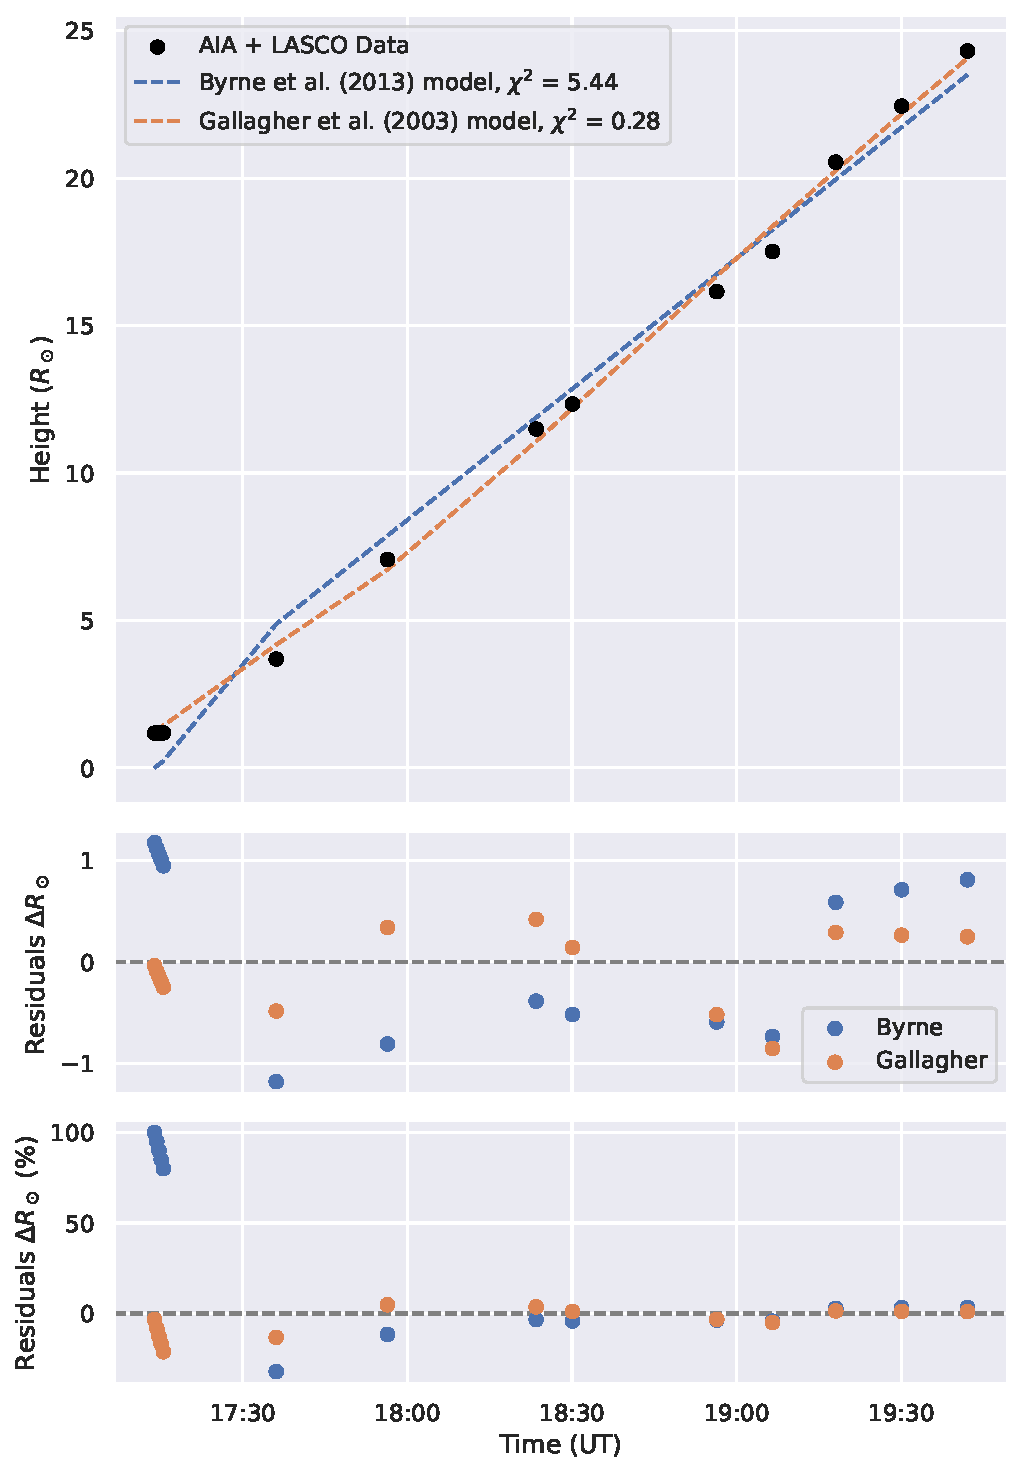
\includegraphics[width=0.8\hsize]{chapter2/figs/appendix/height_profile_residuals_aia_lasco_120313_01.pdf}
	\caption{Same for the event on March 13, 2012.}
\end{figure}

\begin{figure}[!htp]
	\centering
	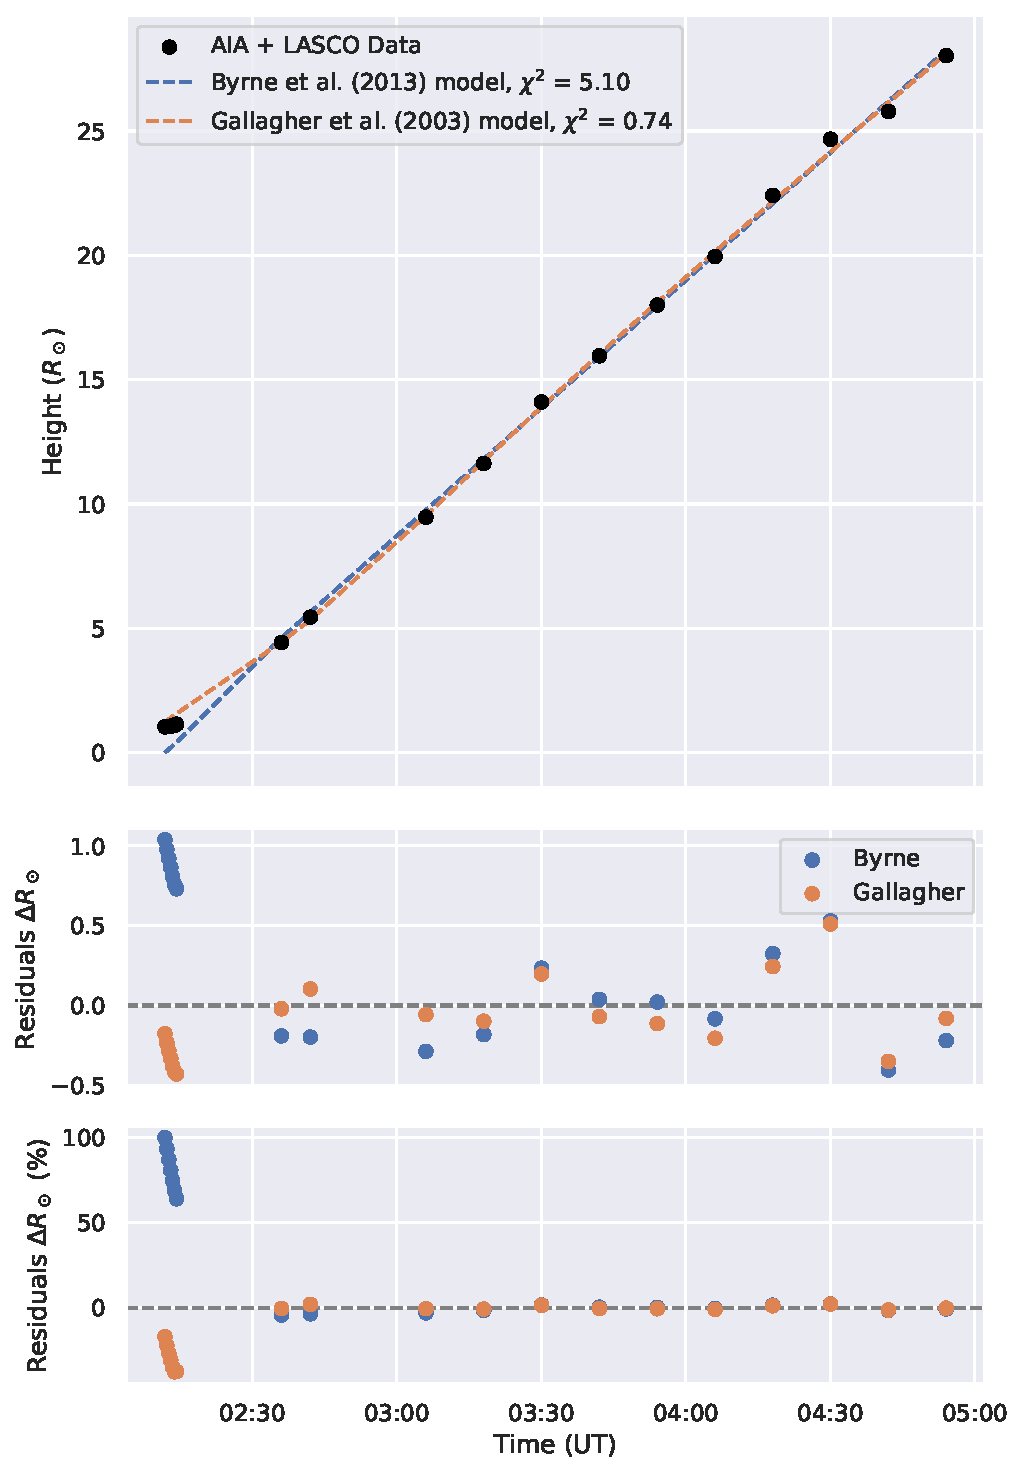
\includegraphics[width=0.8\hsize]{chapter2/figs/appendix/height_profile_residuals_aia_lasco_120723_01.pdf}
	\caption{Same for the event on July 23, 2012.}
\end{figure}

\begin{figure}[!htp]
	\centering
	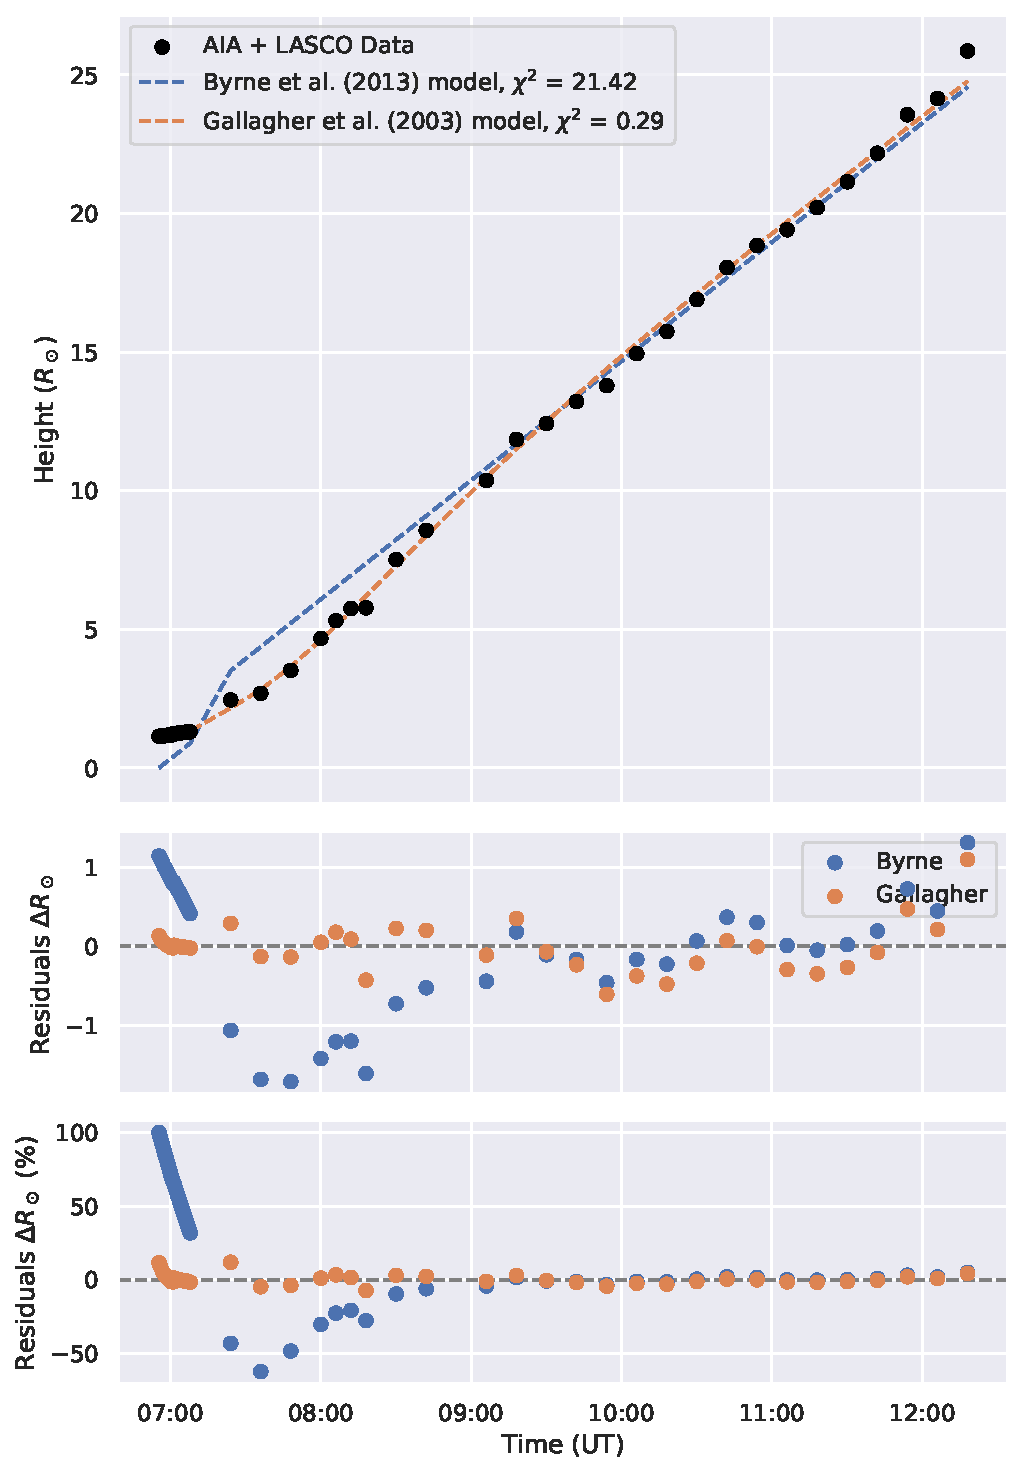
\includegraphics[width=0.8\hsize]{chapter2/figs/appendix/height_profile_residuals_aia_lasco_130421_01.pdf}
	\caption{Same for the event on April 21, 2013.}
\end{figure}

\begin{figure}[!htp]
	\centering
	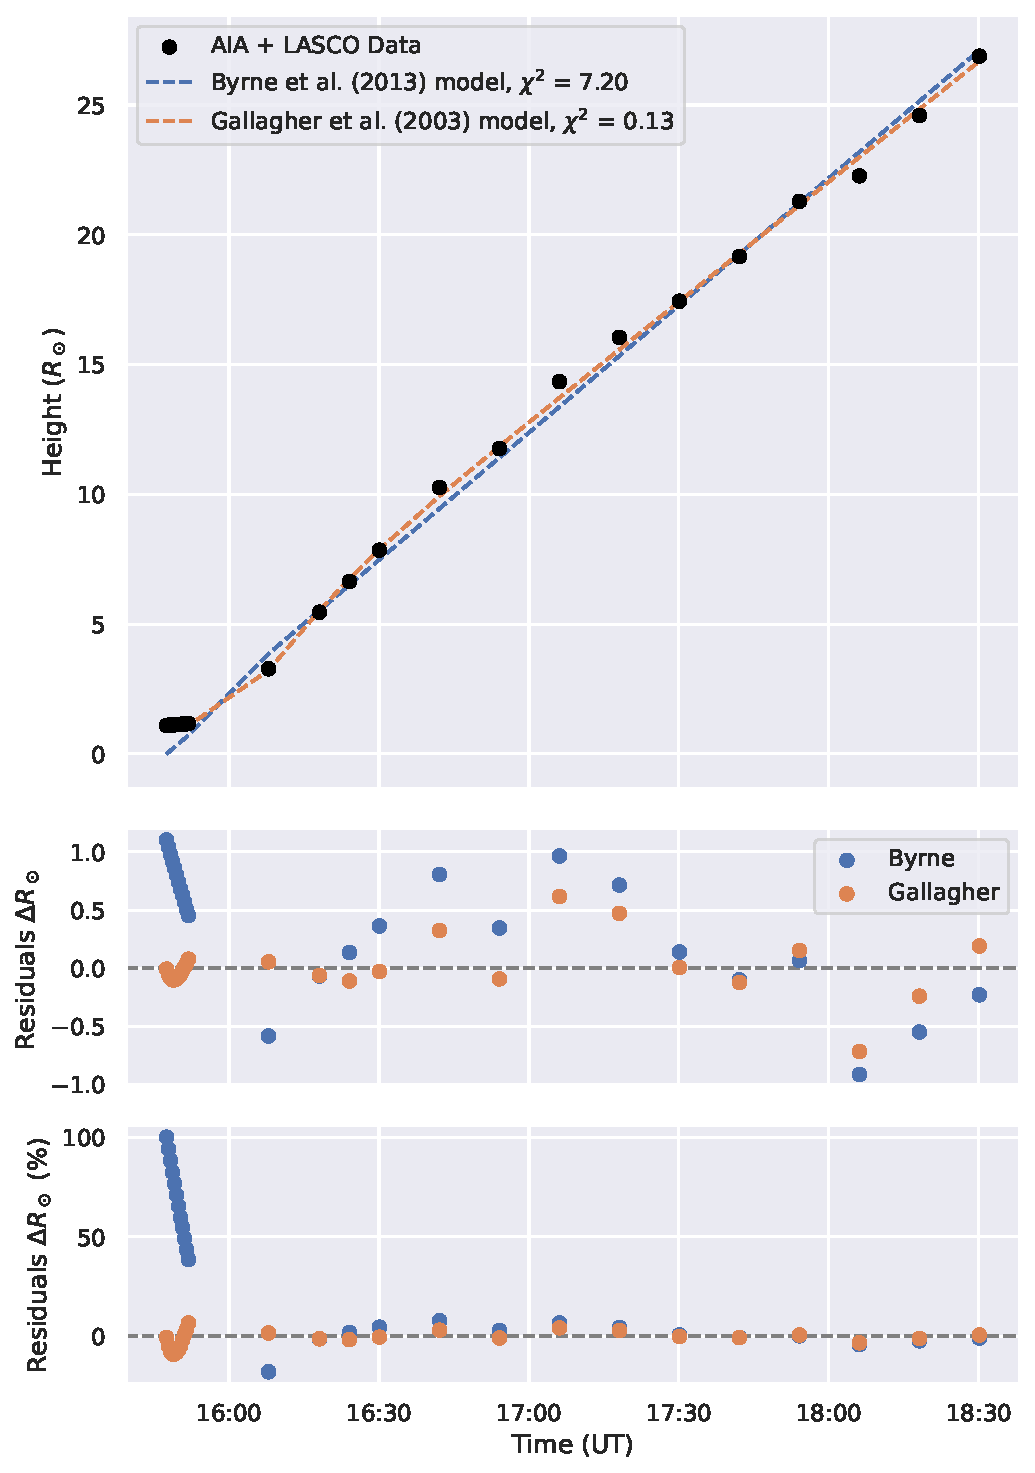
\includegraphics[width=0.8\hsize]{chapter2/figs/appendix/height_profile_residuals_aia_lasco_130513_01.pdf}
	\caption{Same for the event on May 13, 2013.}
\end{figure}

\begin{figure}[!htp]
	\centering
	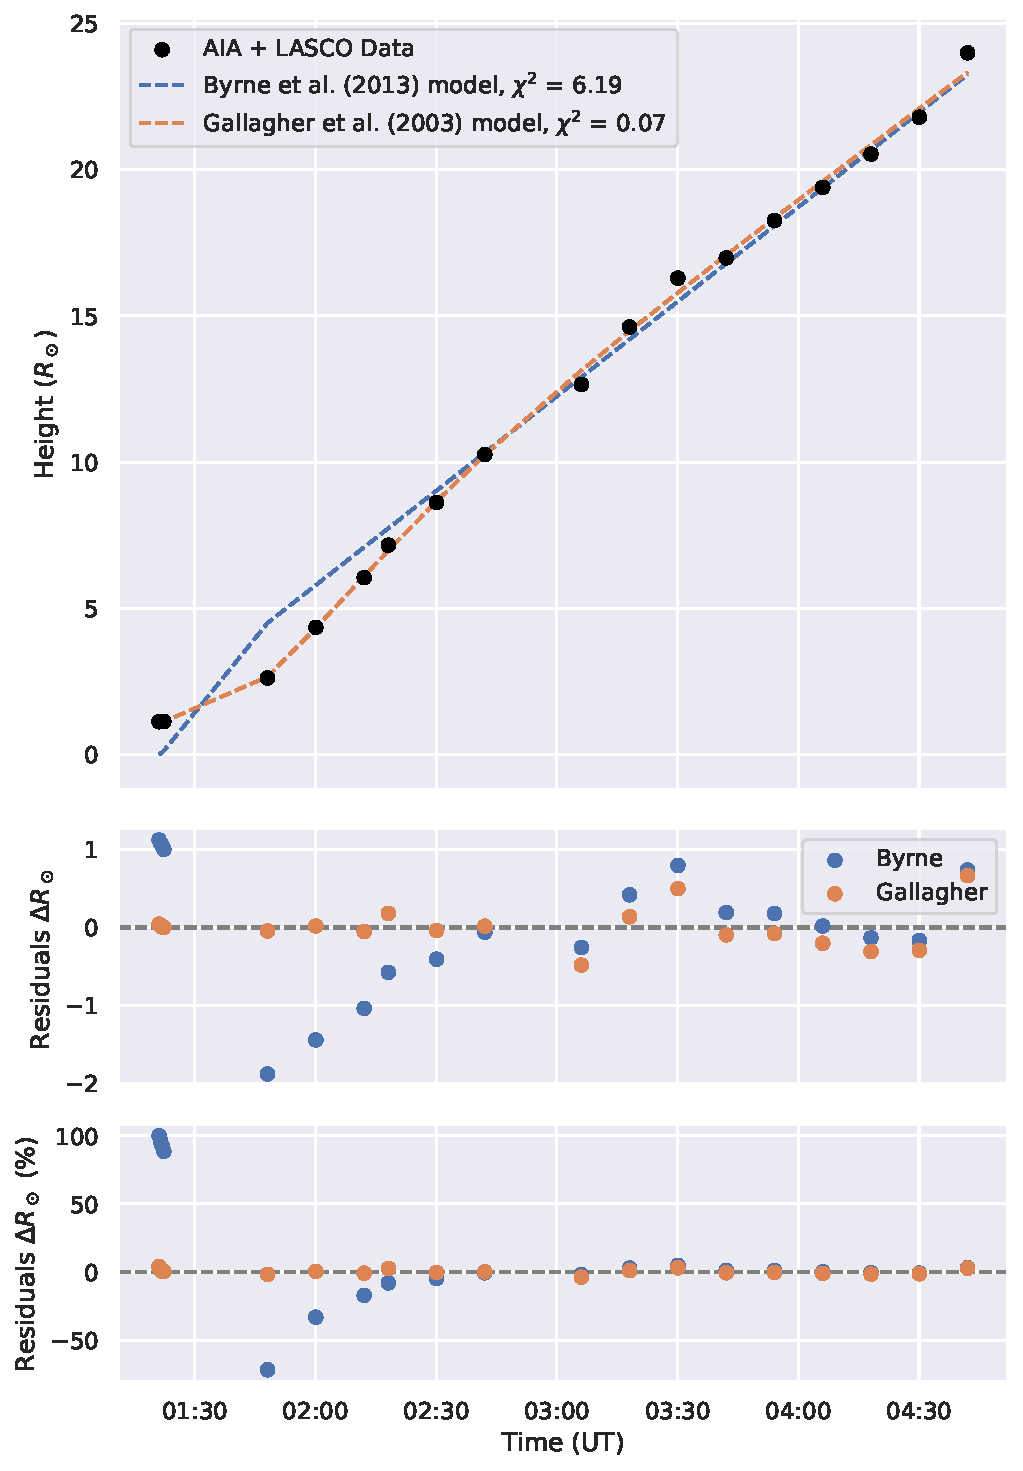
\includegraphics[width=0.8\hsize]{chapter2/figs/appendix/height_profile_residuals_aia_lasco_130515_01.pdf}
	\caption{Same for the event on May 15, 2013.}
\end{figure}

\begin{figure}[!htp]
	\centering
	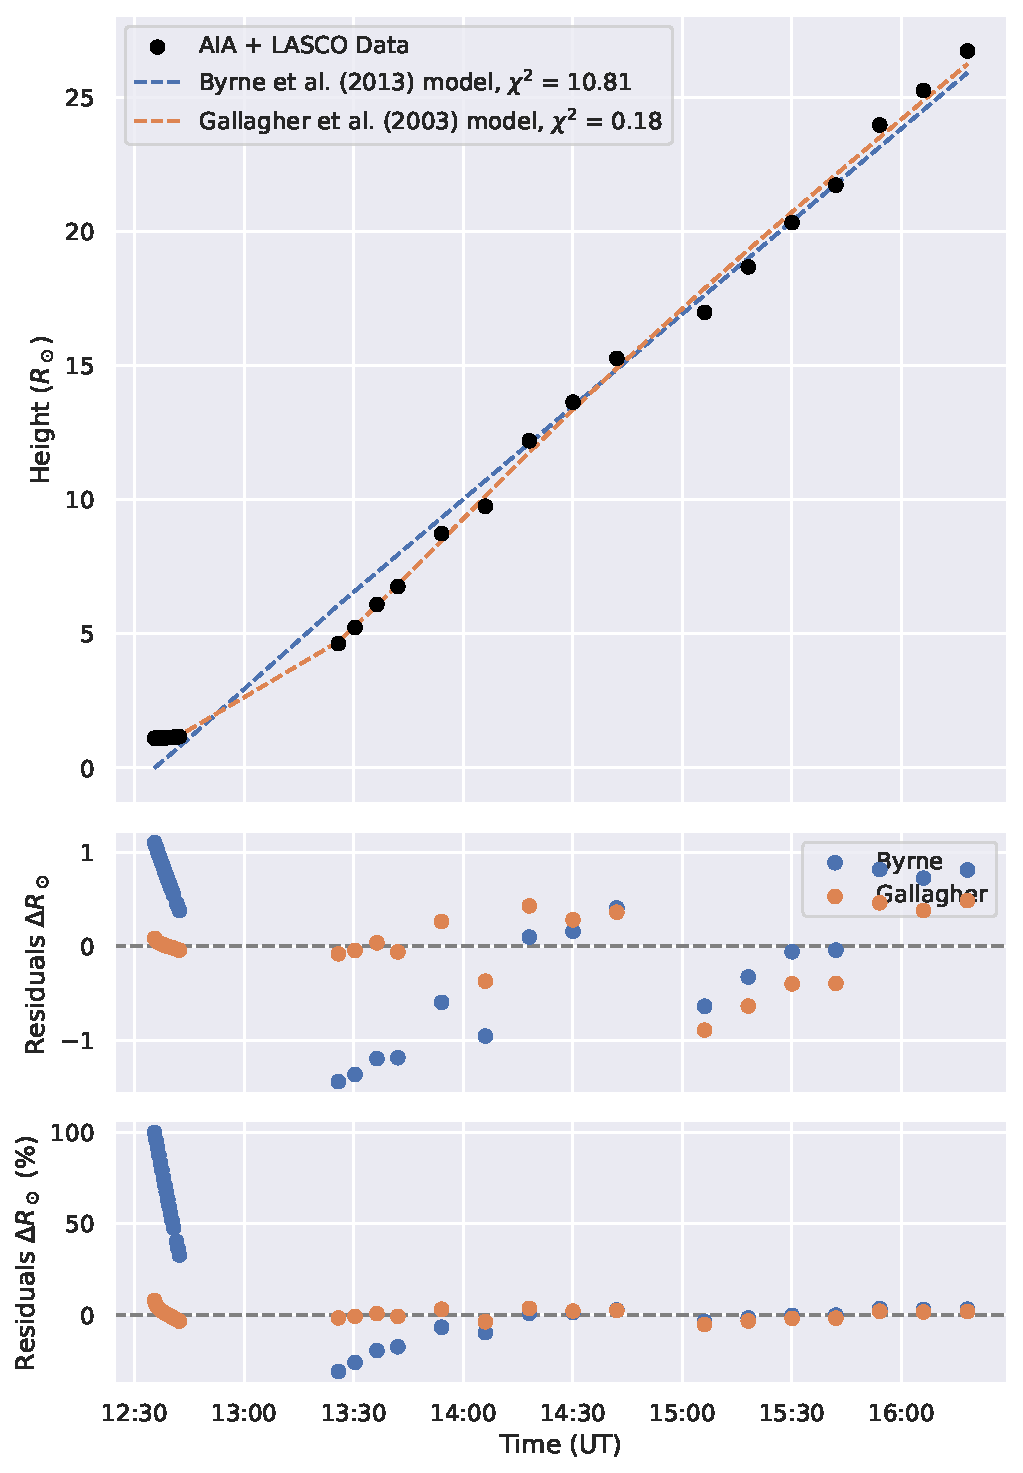
\includegraphics[width=0.8\hsize]{chapter2/figs/appendix/height_profile_residuals_aia_lasco_130522_01.pdf}
	\caption{Same for the event on May 22, 2013.}
\end{figure}

\begin{figure}[!htp]
	\centering
	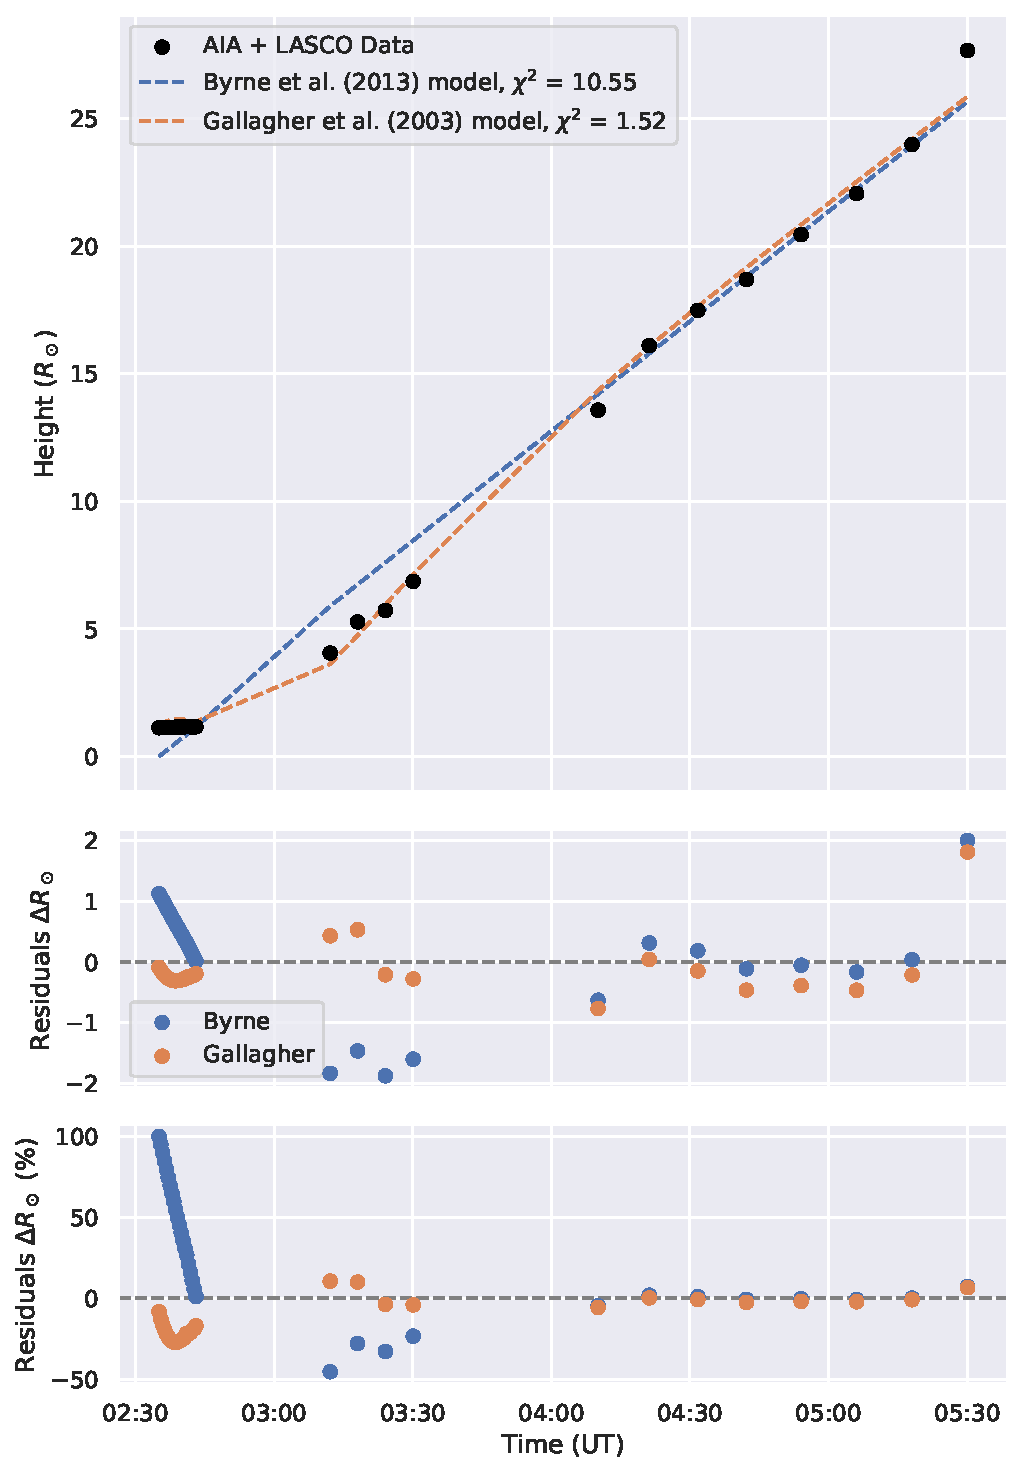
\includegraphics[width=0.8\hsize]{chapter2/figs/appendix/height_profile_residuals_aia_lasco_130621_01.pdf}
	\caption{Same for the event on June 21, 2013.}
\end{figure}

\begin{figure}[!htp]
	\centering
	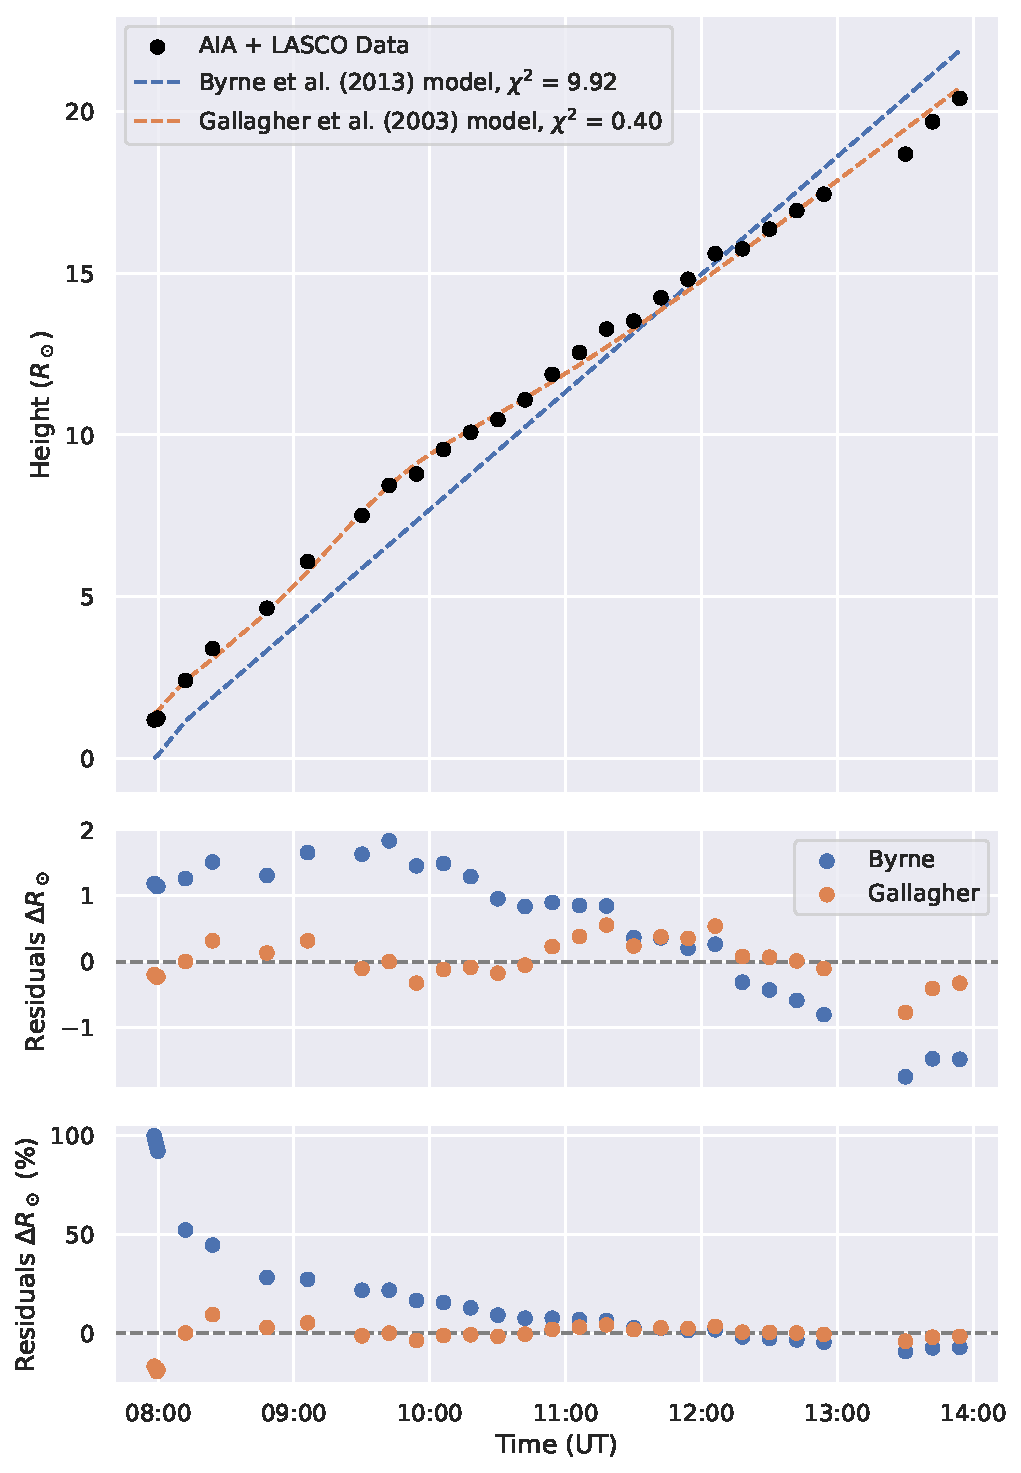
\includegraphics[width=0.8\hsize]{chapter2/figs/appendix/height_profile_residuals_aia_lasco_131025_01.pdf}
	\caption{Same for the event on October 25, 2013.}
\end{figure}

\begin{figure}[!htp]
	\centering
	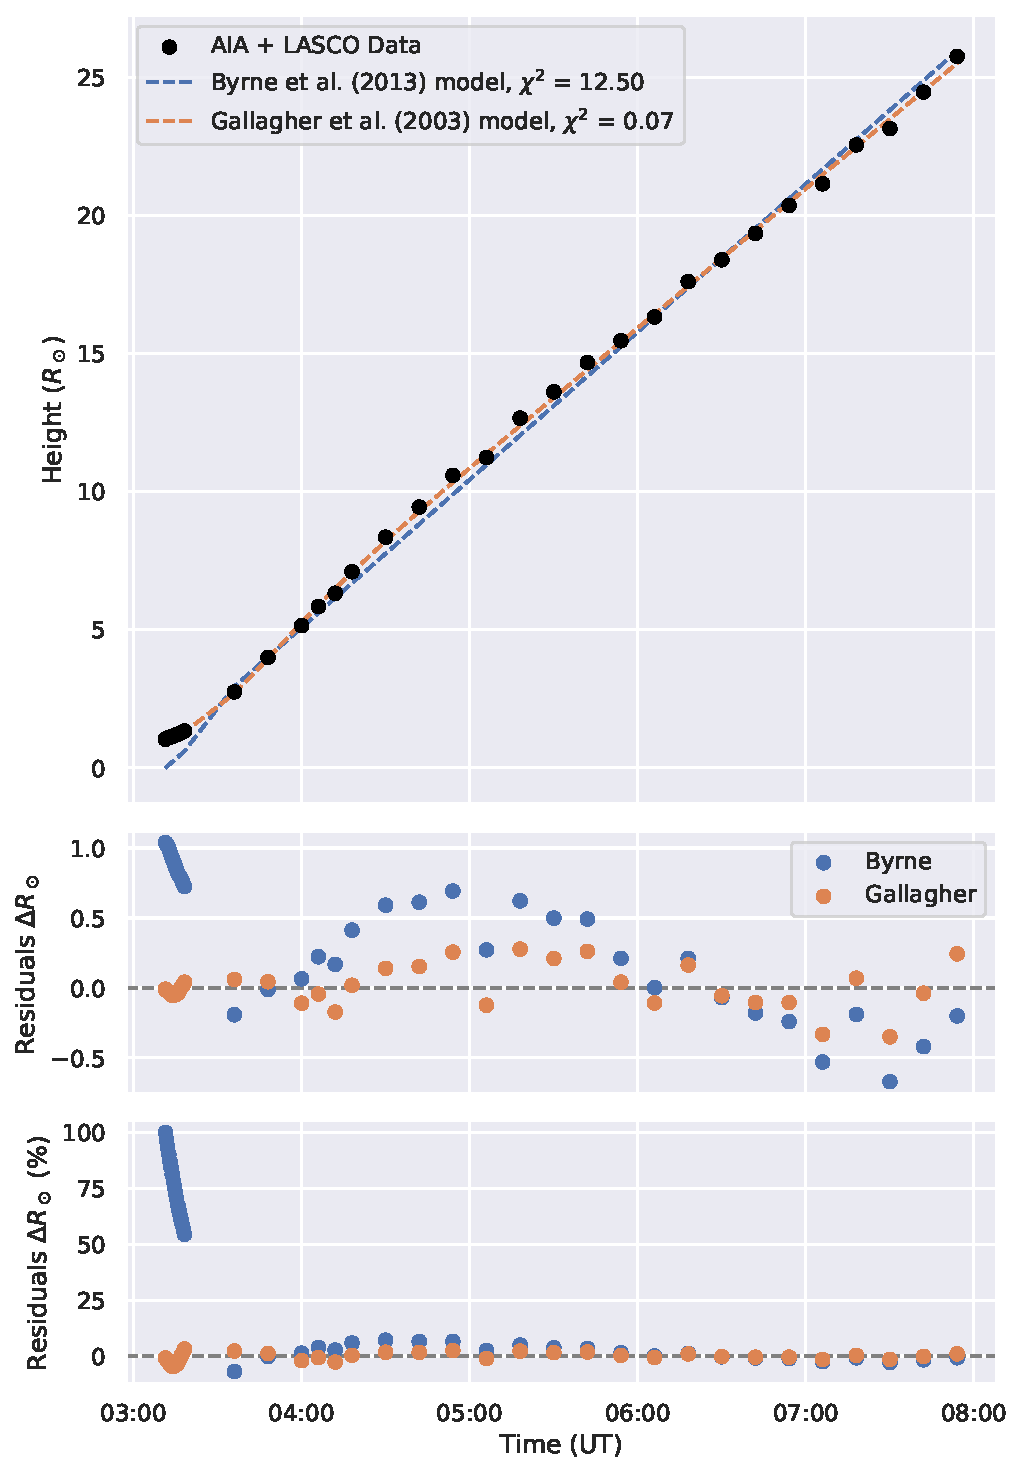
\includegraphics[width=0.8\hsize]{chapter2/figs/appendix/height_profile_residuals_aia_lasco_131212_01.pdf}
	\caption{Same for the event on December 12, 2013.}
\end{figure}

\begin{figure}[!htp]
	\centering
	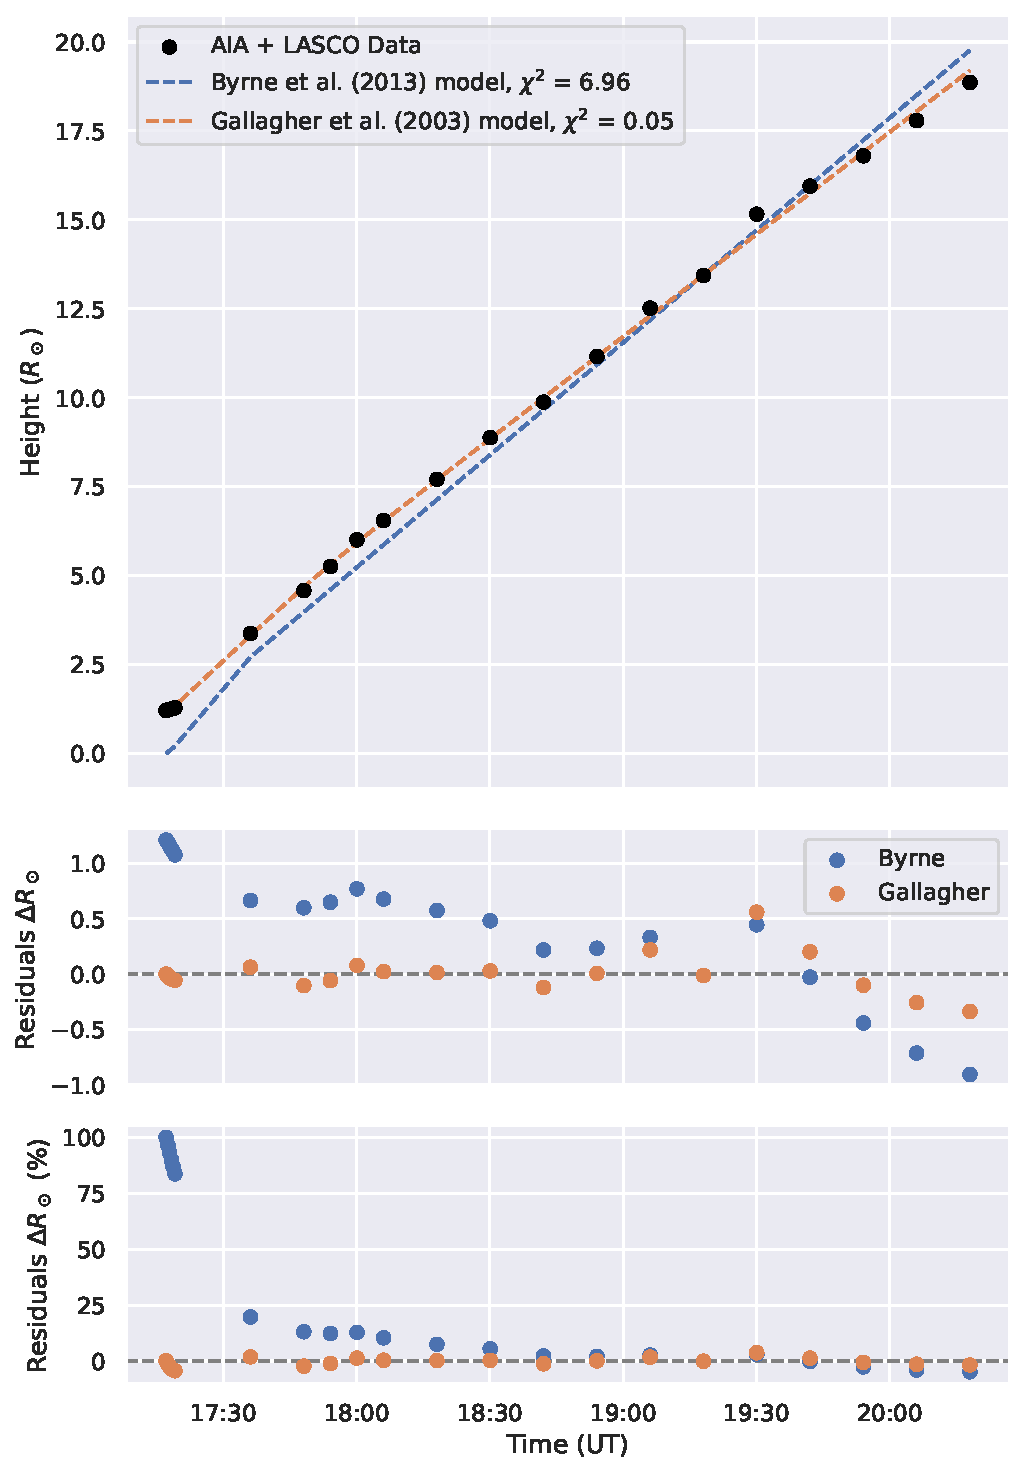
\includegraphics[width=0.8\hsize]{chapter2/figs/appendix/height_profile_residuals_aia_lasco_131228_01.pdf}
	\caption{Same for the event on December 28, 2013.}
\end{figure}

\begin{figure}[!htp]
	\centering
	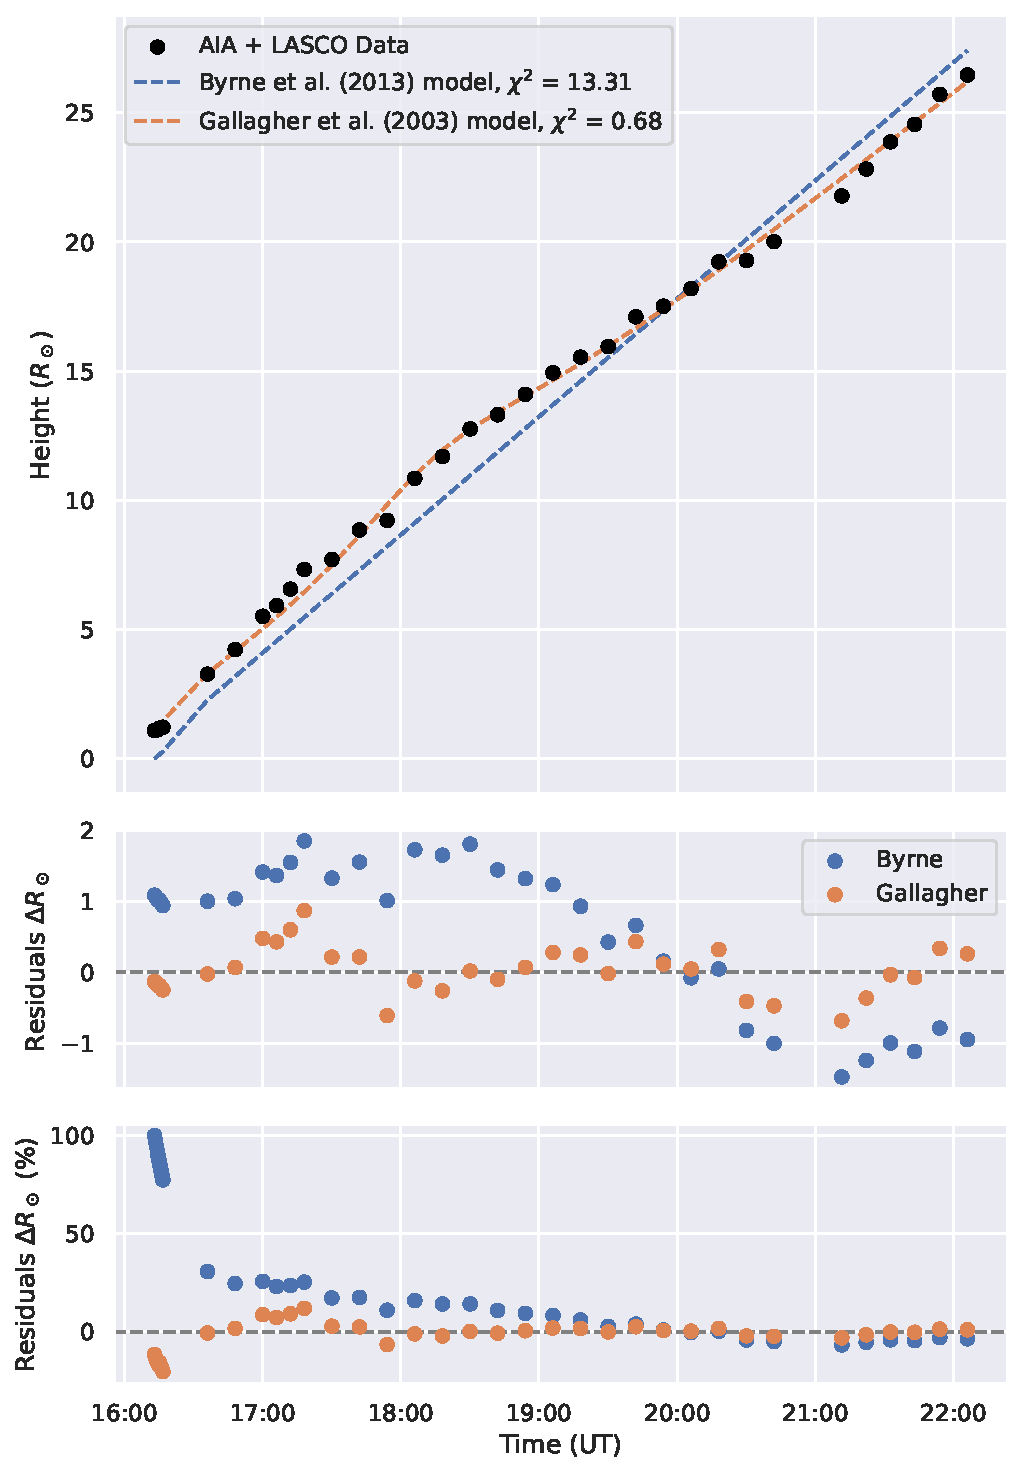
\includegraphics[width=0.8\hsize]{chapter2/figs/appendix/height_profile_residuals_aia_lasco_140708_01.pdf}
	\caption{Same for the event on July 8, 2014.}
\end{figure}

\begin{figure}[!htp]
	\centering
	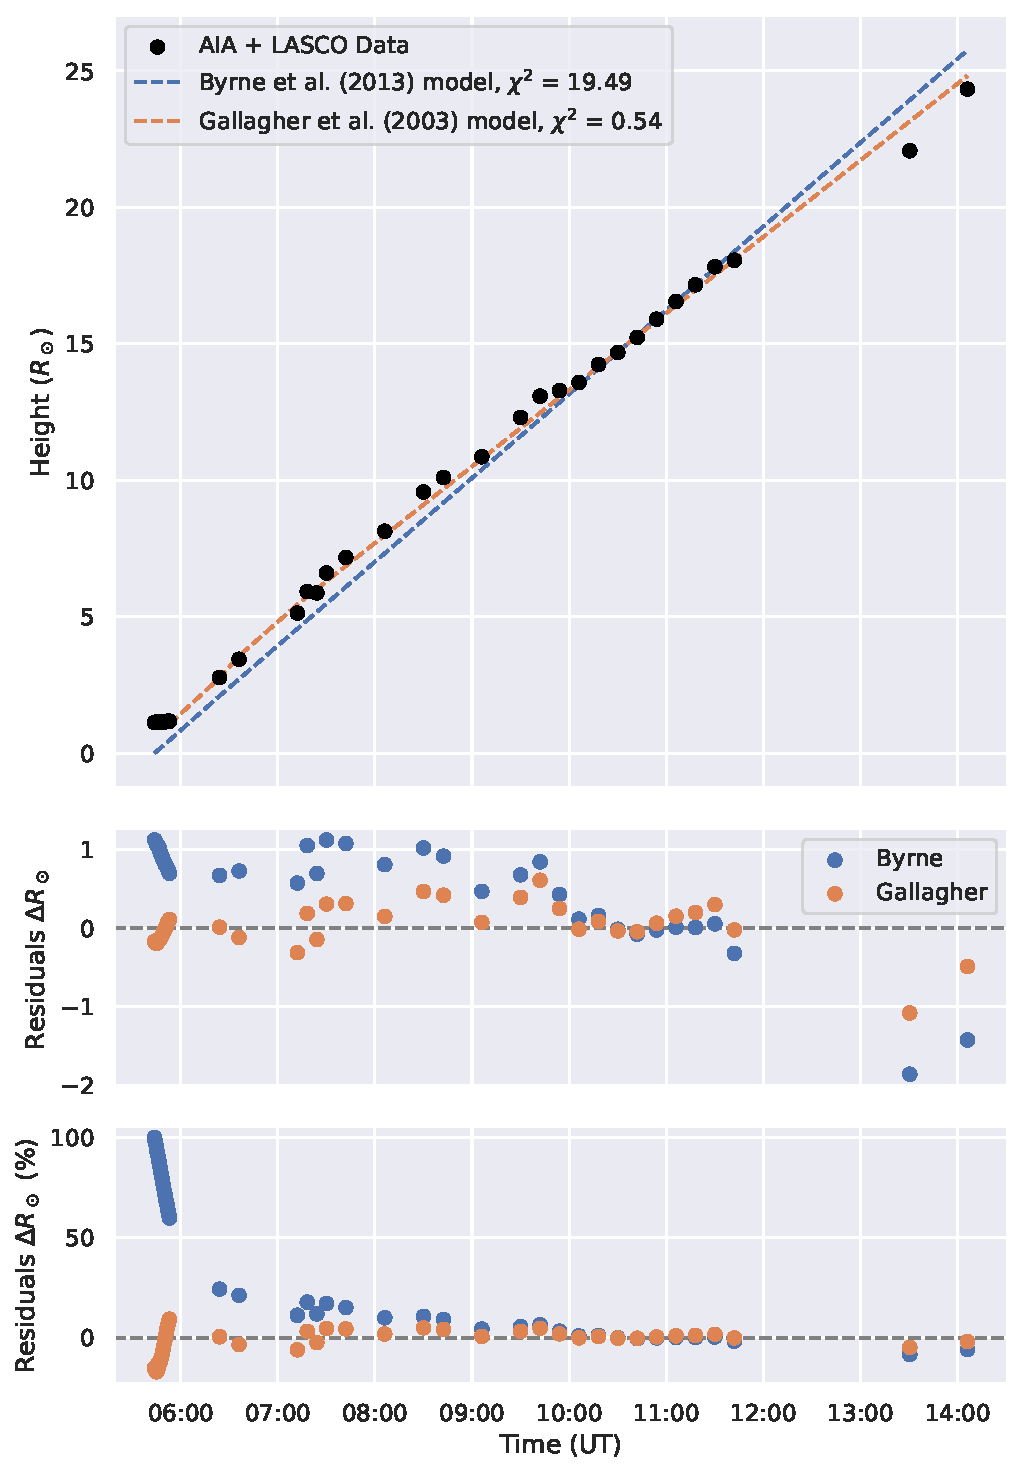
\includegraphics[width=0.8\hsize]{chapter2/figs/appendix/height_profile_residuals_aia_lasco_141205_01.pdf}
	\caption{Same for the event on December 5, 2014.}
\end{figure}

\begin{figure}[!htp]
	\centering
	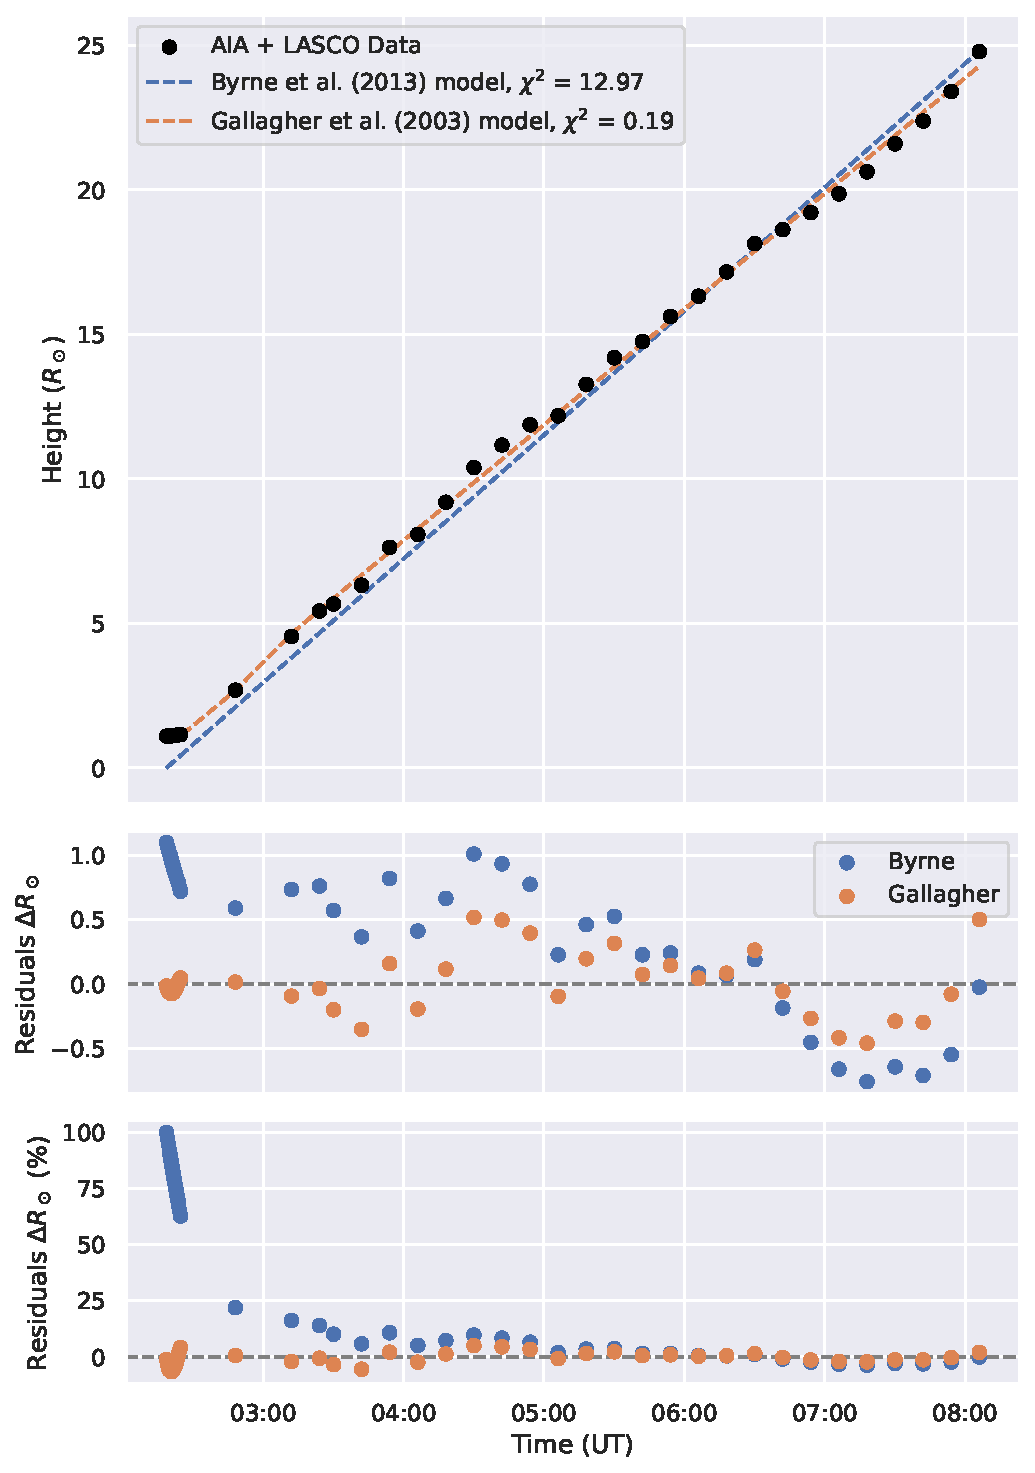
\includegraphics[width=0.8\hsize]{chapter2/figs/appendix/height_profile_residuals_aia_lasco_150512_01.pdf}
	\caption{Same for the event on May 12, 2015.}
\end{figure}

\begin{figure}[!htp]
	\centering
	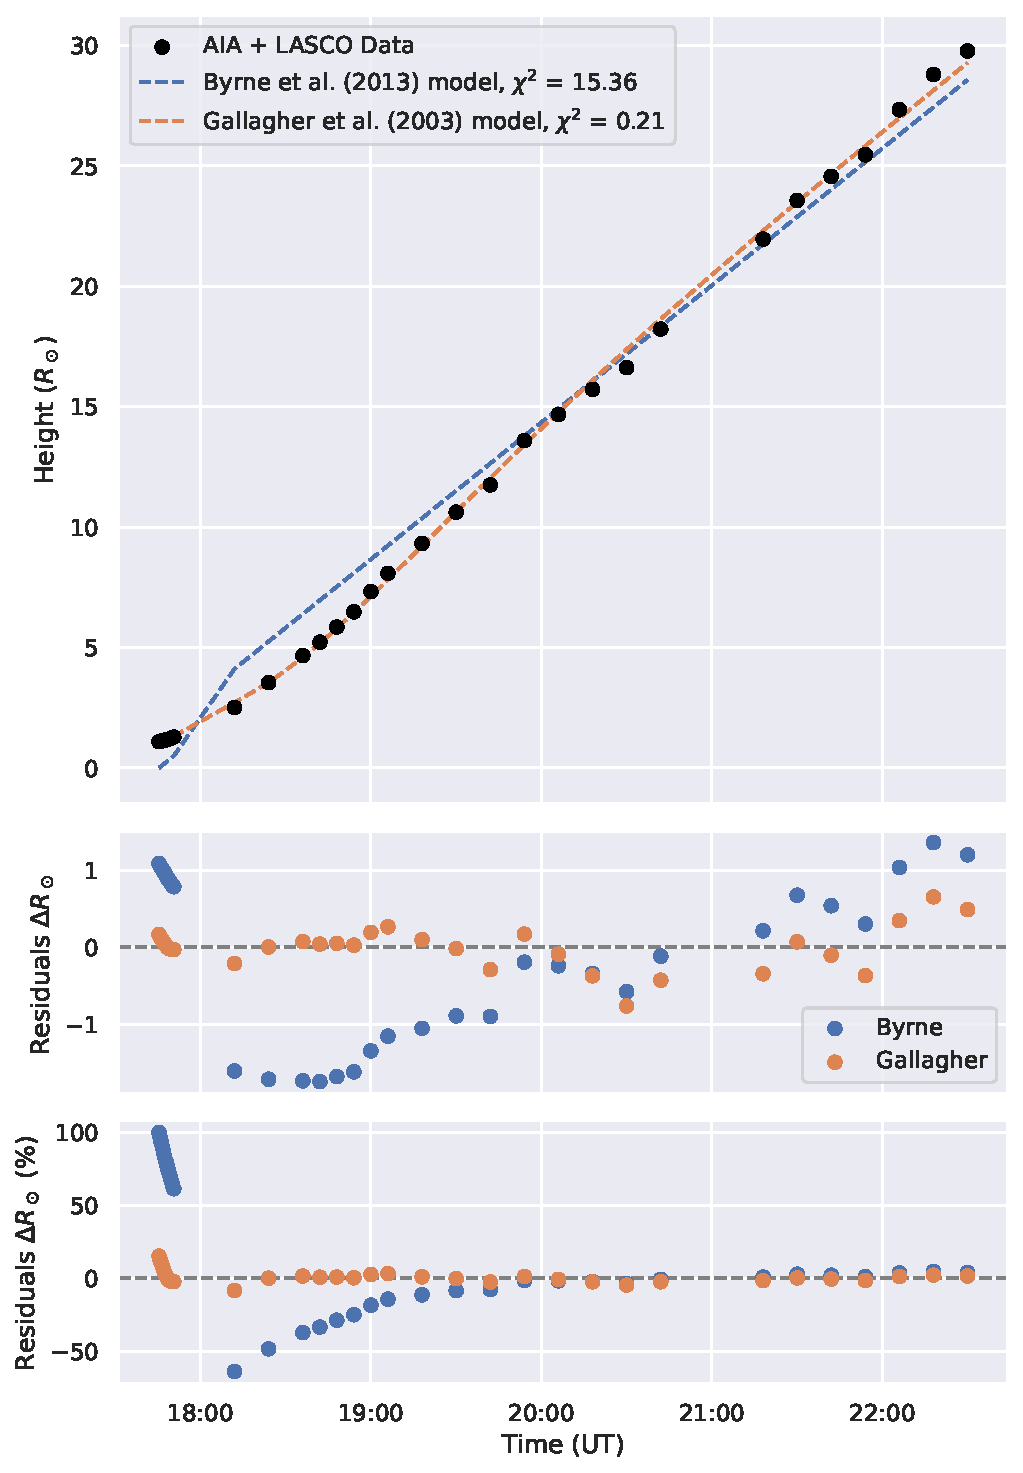
\includegraphics[width=0.8\hsize]{chapter2/figs/appendix/height_profile_residuals_aia_lasco_150920_01.pdf}
	\caption{Same for the event on September 20, 2015.}
\end{figure}

\begin{figure}[!htp]
	\centering
	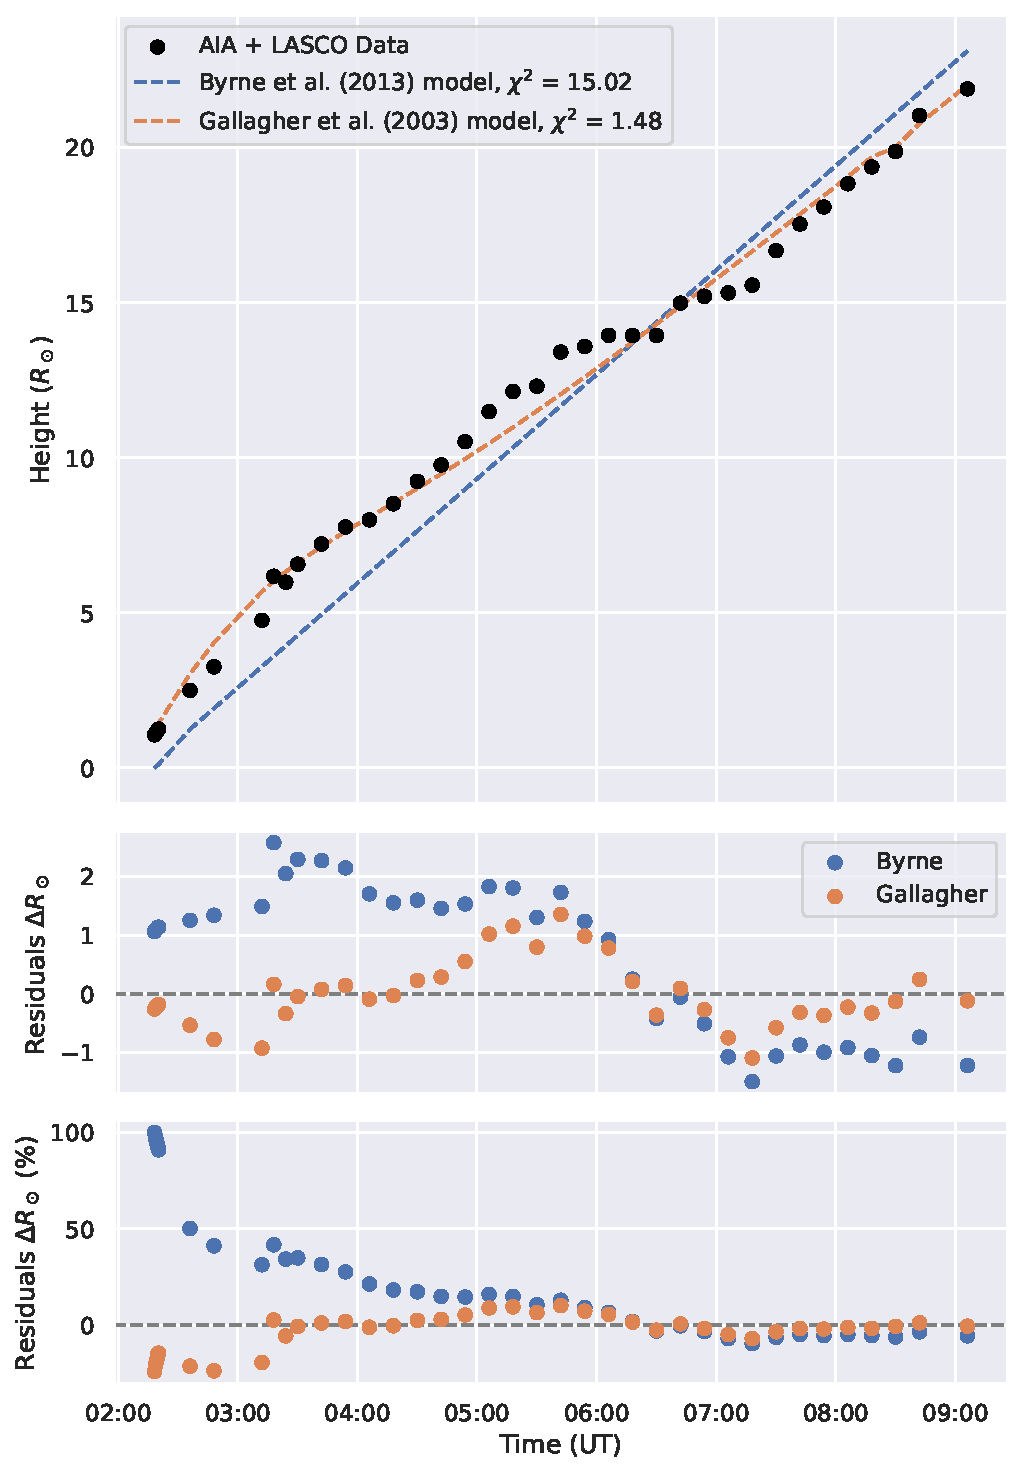
\includegraphics[width=0.8\hsize]{chapter2/figs/appendix/height_profile_residuals_aia_lasco_151029_01.pdf}
	\caption{Same for the event on October 29, 2015.}
\end{figure}

\begin{figure}[!htp]
	\centering
	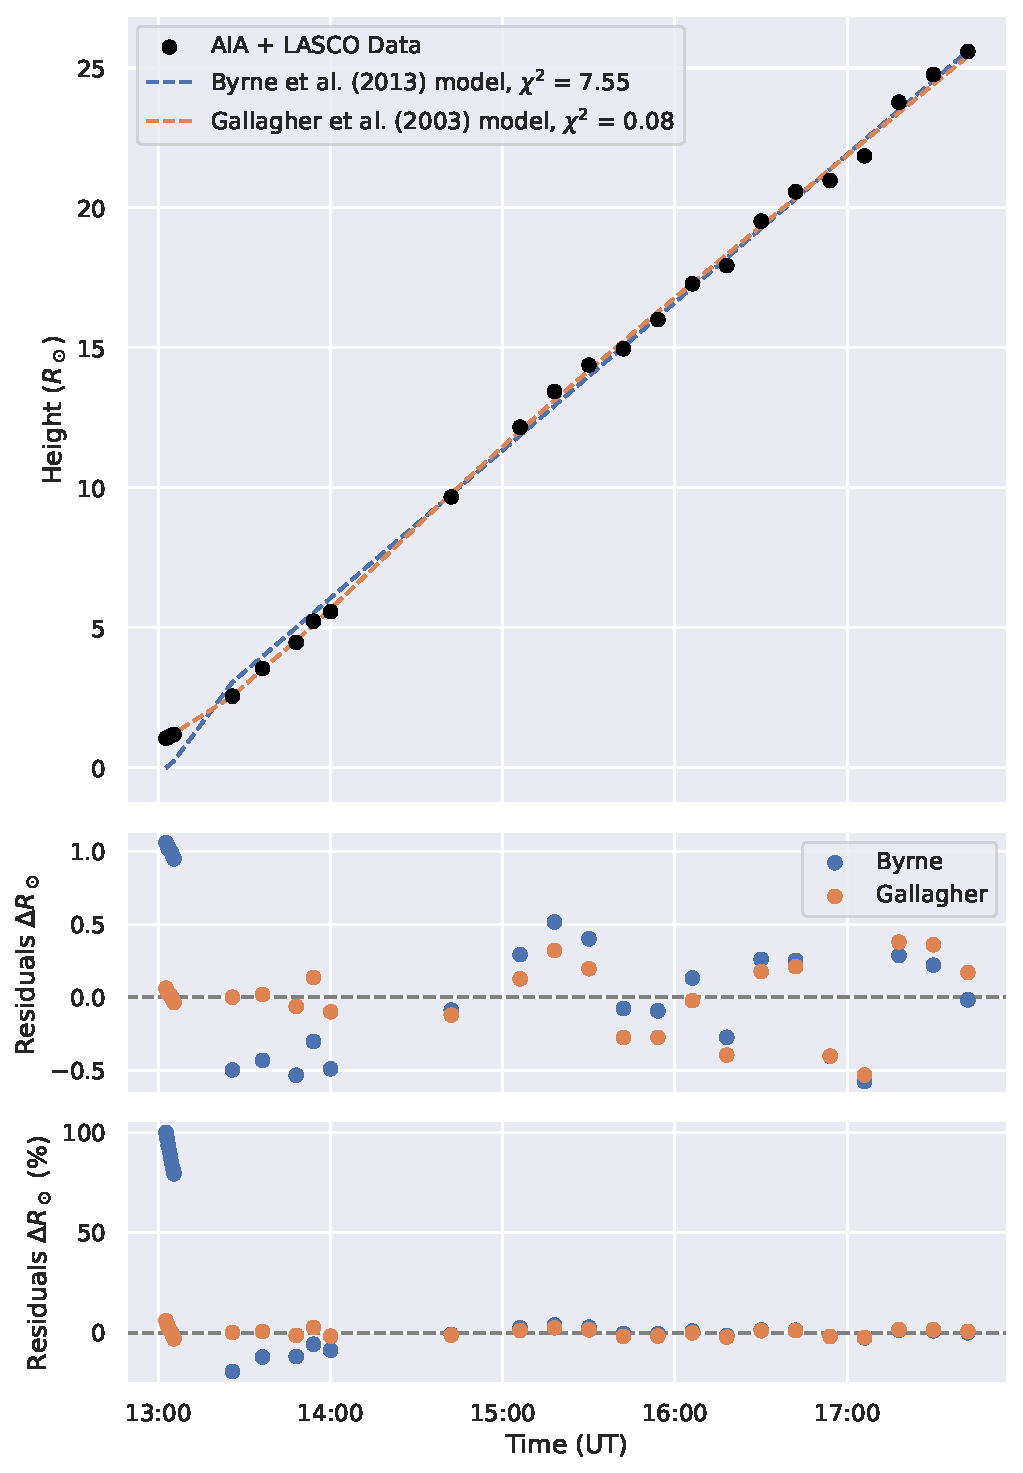
\includegraphics[width=0.8\hsize]{chapter2/figs/appendix/height_profile_residuals_aia_lasco_151109_01.pdf}
	\caption{Same for the event on November 9, 2015.}
\end{figure}

\begin{figure}[!htp]
	\centering
	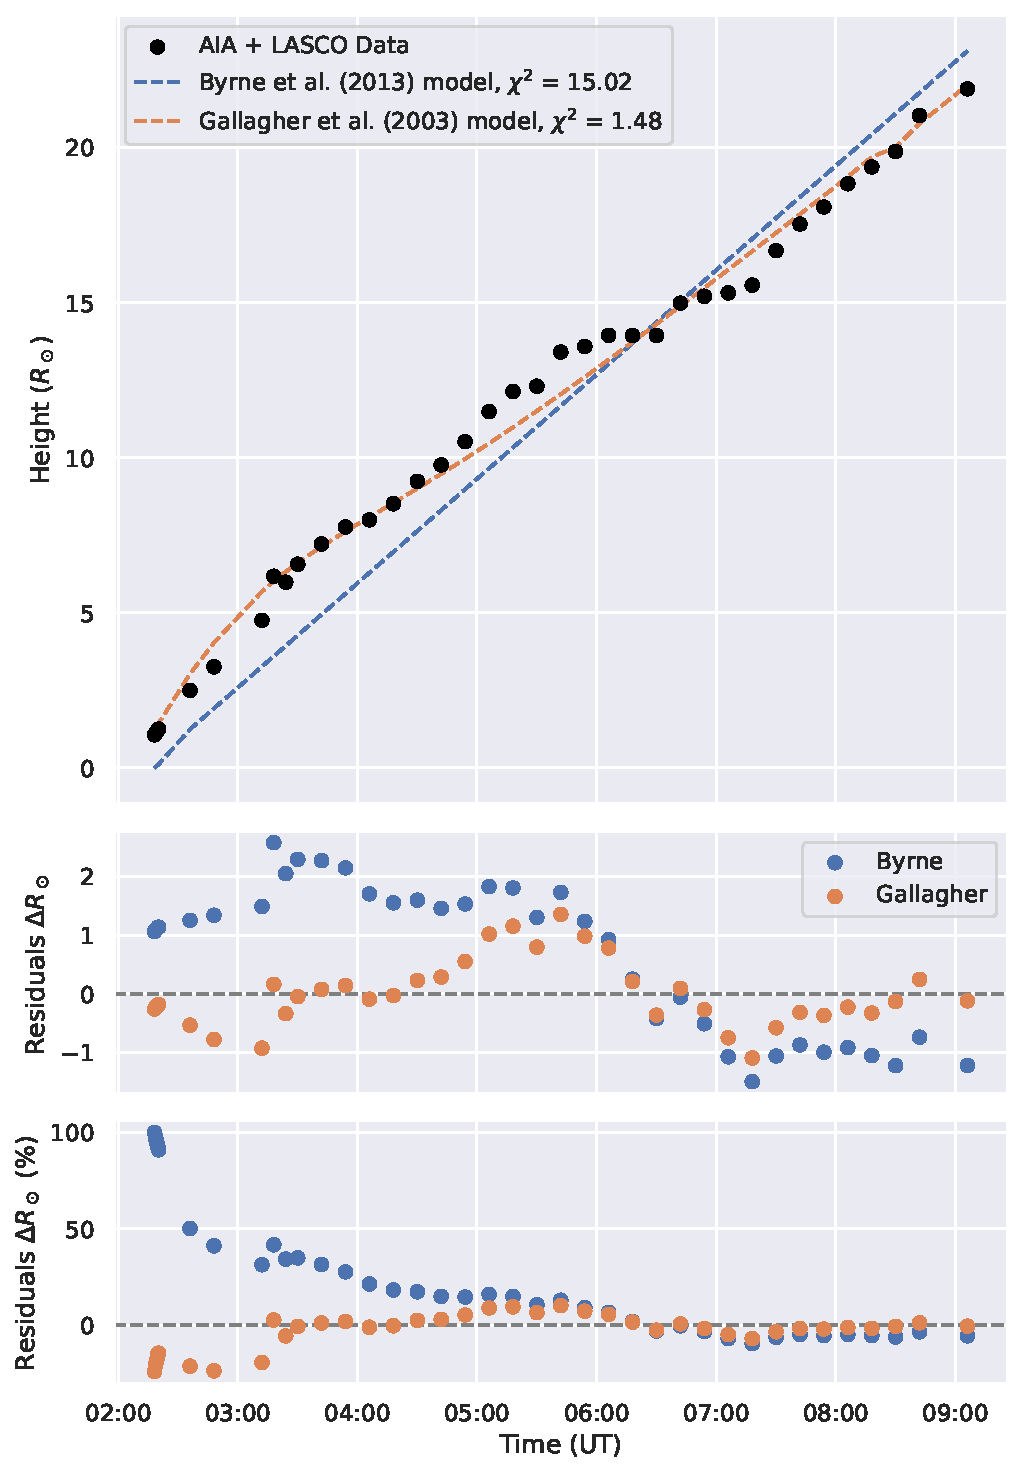
\includegraphics[width=0.8\hsize]{chapter2/figs/appendix/height_profile_residuals_aia_lasco_170401_01.pdf}
	\caption{Same for the event on April 1, 2017.}
\end{figure}

\section{Persistent Imaging Technique}
\label{ch3_append_a}
Persistent imaging is a technique used in medical imaging, particularly ultrasound imaging, to create a continuous, real-time display of the anatomy being imaged (see \citeauthor{pysz_2011} \citeyear{pysz_2011}, and references within). The core idea of persistent imaging is to use persistence, or the ability of the human eye to retain an image for a brief moment after it has disappeared to create a more informative and visually clear image \citep{fredkin_1995, thompson_2016}.

At every image in a time-ordered series, the technique keeps the old pixel value if it is brighter than the current pixel value, else it takes the current pixel's value. The result is saved as the current persistence image. Then, the next image in the series is evaluated by comparing it pixel by pixel with respect to the previous persistence image. The resulting image emphasizes the changes between the current image and the previous persistent image, making them more visible to the human eye.

The persistent imaging technique can be described mathematically by a set of equations. If we let $I(t,x,y)$ be the intensity at time $t$ and pixel coordinates $(x,y)$, and let $P(t,x,y)$ be the persistence image at time $t$ and pixel coordinates $(x,y)$, then the persistence image at time $t$ is computed as:
\begin{equation}
	P(t,x,y) = max\{I(t,x,y), P(t-1,x,y)\}
	,\end{equation}
where \textbf{max} represents the maximum of its two arguments. The current image at time $t$ is then evaluated with respect to the previous persistence image as follows:
\begin{equation}
	I^`(t,x,y) = max\{I(t,x,y) - P(t-1,x,y), 0\}
	,\end{equation}
The resulting image $I'(t,x,y)$ is a modified version of the current image that emphasizes the differences from the previous persistence image.

The persistent imaging technique has been shown to improve the visual quality of ultrasound images and other medical imaging modalities, and is commonly used in clinical practice. In this work, I utilize the persistent imaging technique to improve the visualization of the solar radio sources of type III emissions (Fig.~\ref{fig_persistence}).

\section{Resolving the radio emission location ambiguity}
\label{ch3_append_b}
In this part, we show that the -Z solution of Equation~\ref{zpos} is highly unlikely in our case. Figure~\ref{fig_negZ_posZ} shows the positive and negative solutions of Equation~\ref{zpos}. I take the innermost and outermost coronal radio sources at $R_1$ and $R_2$, respectively, as an example. $r_1$ and $r_2$ are the projections of $R_1$ and $R_2$ on the POS, respectively. Harmonic radio emission from $R_1$ will theoretically be absorbed by a region along the LOS with plasma frequency (and corresponding density) equal to or higher than the harmonic emission frequency at $R_1$. In the case of the spherically symmetric Newkirk model, the highest density location the emission from $R_1$ could pass through is $r_1$ on the POS. Thus, for harmonic radio emission from behind the POS (-Z, where Z = 0 is defined at the center of the Sun and positive Z is towards the observer) to be observed at the Earth, it must satisfy the following condition:
\begin{equation}
	2f_{R_1} > f_{r_1}
	\label{eq_assumption}
	,\end{equation}
where $f_{R_1}$ is the plasma frequency of radio emission that occurred behind the POS, and $f_{r_1}$ is the plasma frequency at the projected location of $r_1$ on the POS.
The relation between the local plasma frequency and the electron density is defined by the equation:
\begin{equation}
	f[MHz] = 8.93 \times 10^{-3} \sqrt{n[cm^{-3}]}
	\label{eq_plasmafreq}
	.\end{equation}
The Newkirk electron-density model \citep{newkirk_1961, newkirk_1967} describes the typical densities in the outer part of the corona according to the following equation:
\begin{equation}
	n[cm^{-3}] = \alpha \; 4.2 \times 10^4 \; 10^{4.32 \frac{R_\odot}{r}}
	\label{eq_newkirk}
	,\end{equation}
where $\alpha$ is the fold number (i.e., a multiplicative factor that accounts for the density variations based on the degree of solar activity), and $r$ is the radial distance from the Sun in solar radii.
By substituting Equations~\ref{eq_plasmafreq} and~\ref{eq_newkirk} into Equation~\ref{eq_assumption}, we obtain
\begin{equation}
	\frac{n_{r_1}}{n_{R_1}} = \frac{10^{4.32 \frac{R_\odot}{r_1}}}{10^{4.32 \frac{R_\odot}{R_1}}} < 4.
	\label{eq_condition}
\end{equation}
After reduction we obtain the final formula that must be satisfied under these assumptions in order for radio emission behind the POS to pass through the corona and reach the Earth:
\begin{equation}
	\frac{r_1}{R_\odot} < \left( \frac{log 2}{2.16} + \frac{R_\odot}{R_1} \right)^{-1}.
\end{equation}

\begin{figure}[h!]
	\centering
	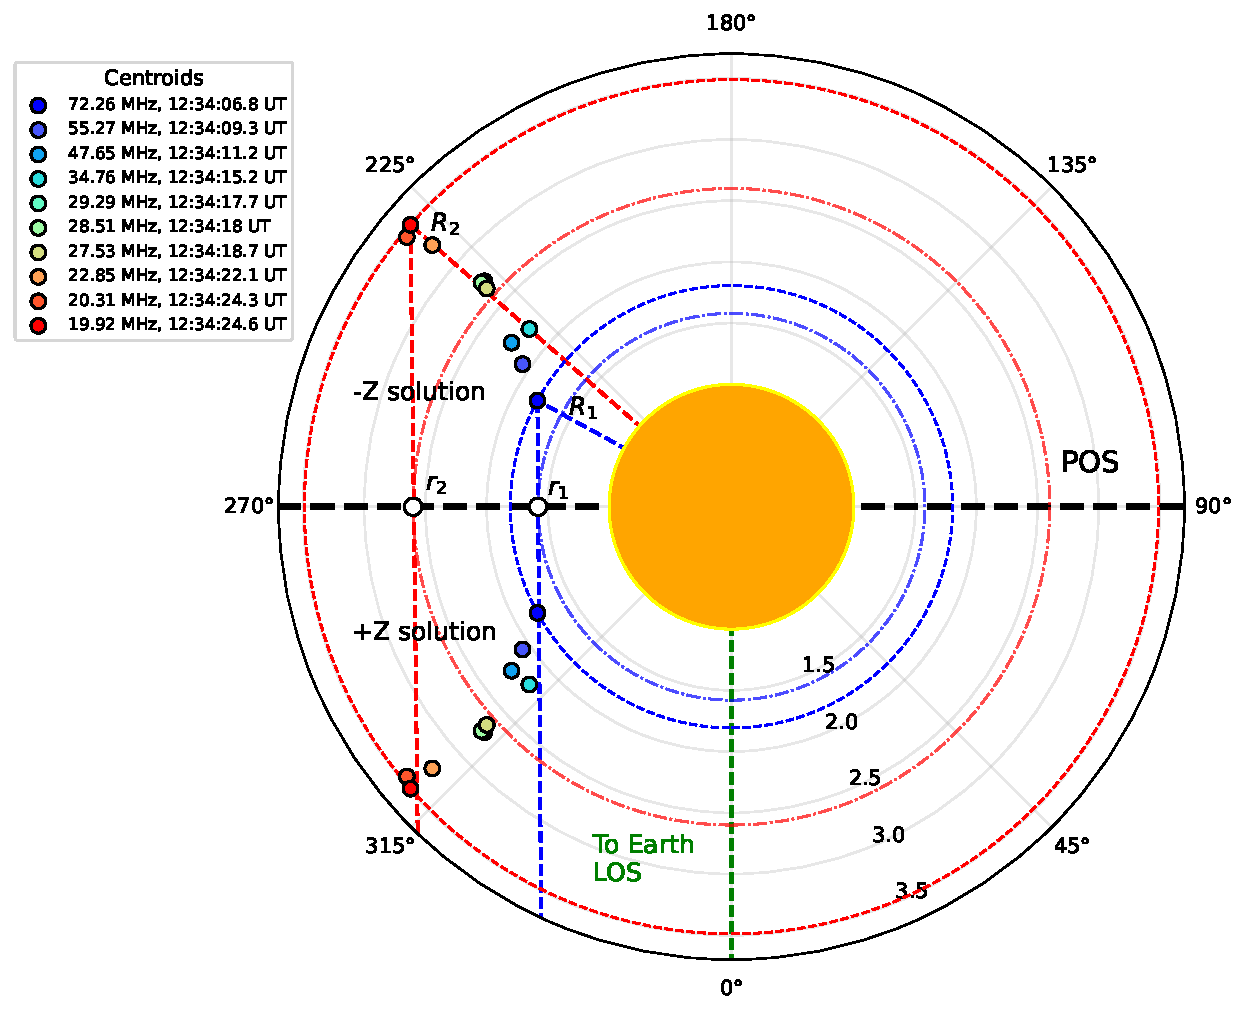
\includegraphics[width=0.8\hsize]{chapter3/figs/negZ_posZ_solutions.pdf}
	\caption{Schematic shows the locations of the radio sources for the +Z and -Z solutions of Equation~\ref{zpos}. The Sun is located in the middle as an orange circle, with a horizontal dashed black line representing the POS. The vertical dashed green line represents the Sun-Earth LOS. The dashed blue and red circles represent the plasma spheres of density equivalent to the observation frequencies of the innermost and outermost radio sources at $R_1$ and $R_2$, respectively, under the Newkirk model assumption of spherically-symmetric density distribution. The impact parameters $r_1$ and $r_2$ are the projection of $R_1$ and $R_2$ on the POS. The dot-dashed blue and red circles are the circles passing through the impact parameters $r_1$ and $r_2$, respectively.}
	\label{fig_negZ_posZ}
\end{figure}
From Figure~\ref{fig_negZ_posZ}, $r_1$ and $r_2$ will always be smaller than $R_1$ and $R_2$, respectively. The Newkirk model requires that the density at $r_1$ and $r_2$ be significantly higher than the density at $R_1$ and $R_2$, respectively (Table~\ref{table_negZ}). Additionally, from the geometric representation in Figure~\ref{fig_negZ_posZ}, we find that the electron density at $r_1$ is higher than at ${R_1}$, hence the radio emission cannot reach the Earth from that point behind the POS \citep{mann_2018}.

From Table~\ref{table_negZ}, the assumption of Equation~\ref{eq_condition} is not satisfied. Thus, the -Z solution is invalid in our case. This implies that the harmonic emission from behind the POS will not reach the Earth. Thus, the +Z assumption is the valid solution.
\begin{table}[h!]
	\centering
	\caption{Radial distances and densities at the first ($R_1$) and last ($R_2$) radio sources were obtained from the 2.5$\times$Newkirk model, as well as their impact parameters $r_1$ and $r_2$, respectively.}
	\label{table_negZ}
	\begin{tabular}{cccc}
		\hline
		Point & Radial distance ($R_\odot$) & Density (cm$^{-3}$) & Ratio ($n_r/n_R$)\\ \hline
		$r_1$ & 1.58 & 5.69$\times10^7$ & \multirow{2}{*}{11.81}\\
		$R_1$ & 1.81 & 4.82$\times10^6$ & \\ \hline
		$r_2$ & 2.6 & 2.59$\times10^7$ & \multirow{2}{*}{14.23}\\
		$R_2$ & 3.49 & 1.82$\times10^6$ & \\ \hline
	\end{tabular}
\end{table}
\begin{figure}
	\centering
	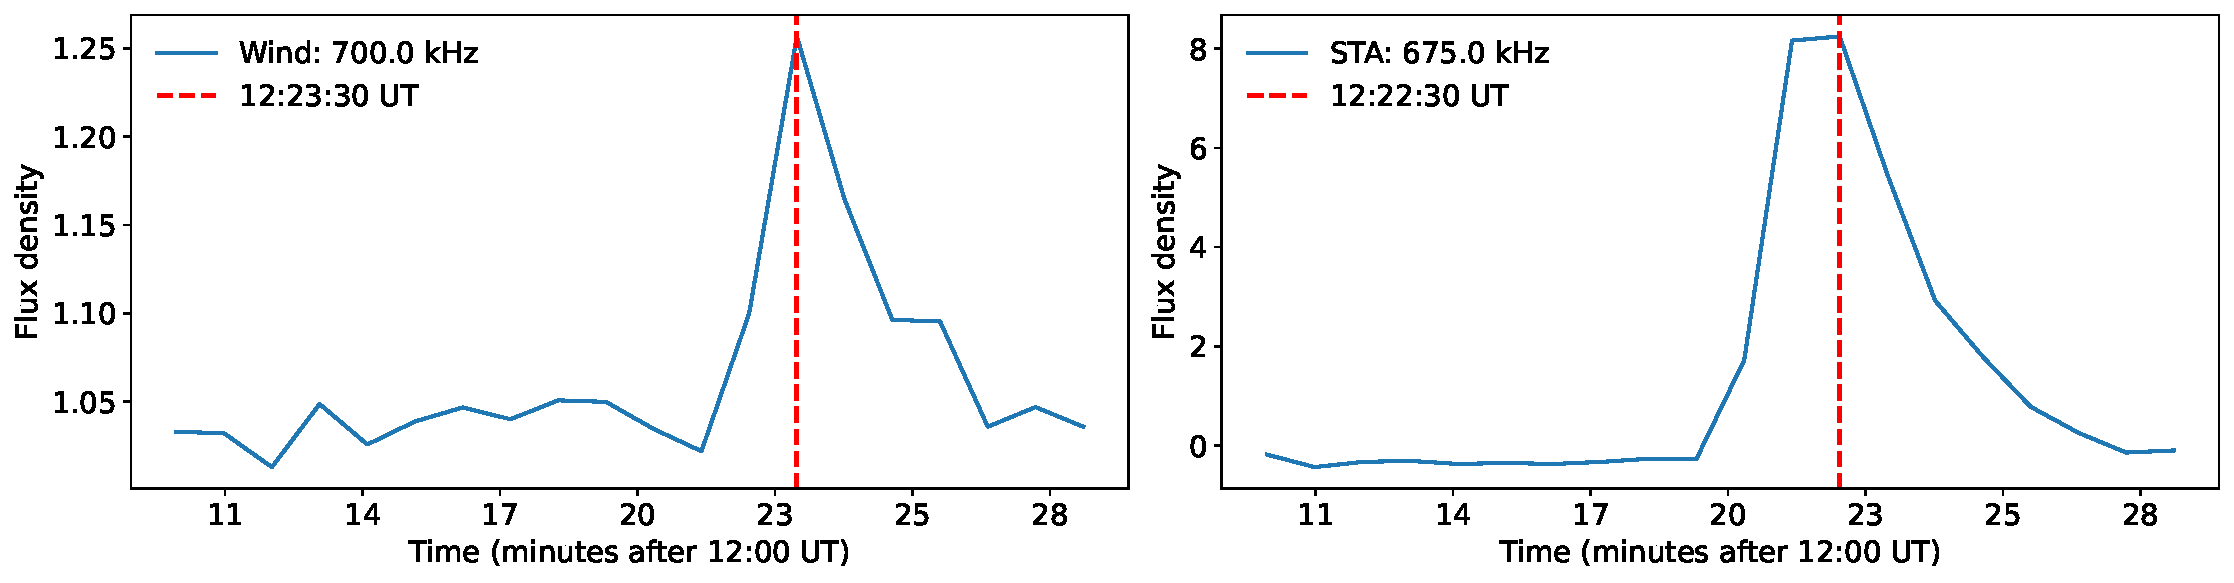
\includegraphics[width=0.9\hsize]{chapter3/figs/wind_vs_sta_fluxdens.pdf}
	\caption{Cut of the flux density at 700 kHz observed by Wind (left panel) and STEREO-A (right panel). Note:\ for STEREO-A, there is no exact frequency channel at 700 kHz; therefore we selected the nearest one (675 kHz).}
	\label{fig_cutpower}
\end{figure}

Furthermore, I analyzed the time difference of arrival of the radio emission at interplanetary wavelengths in Figure~\ref{fig_cutpower}. Specifically, we compared the timing of peak signals at a low frequency between two spacecraft, Wind and STEREO. This analysis was conducted under the assumption of two possible scenarios:
\begin{itemize}
	\item one in which the radio emission source follows a trajectory that is roughly equidistant between Wind and STEREO -- if the $+Z$ assumption is true.
	\item the trajectory implies significantly longer travel times from the source to Wind compared to STEREO -- if the $-Z$ assumption is true.
\end{itemize}
Examining the data, I selected the frequency channel 700 kHz observed by Wind and its nearest counterpart 675 kHz for STEREO. Interestingly, the difference in the arrival times of these signals was merely one minute, which is within the bounds of the time resolution of the instrument. This negligible difference in arrival times supports the $+Z$ assumption for the beam trajectory, meaning it travels approximately at an equal distance between the two spacecraft.

%\section{Appendic for SEP-related Work}}
%\label{ch4_appendix_eval}

\section{Machine Learning Terminologies}
\label{terminologies_appendix}
In this section, I introduce the main concepts related to machine learning which are presented in the dissertation.

\begin{itemize}
    \item \textbf{Cross-validation}: A technique used to evaluate the performance of a machine learning model by dividing the data into subsets and assessing the model on different combinations of these subsets.

    \item \textbf{Input Horizon}: The number of previous time steps considered as input to a model for time series forecasting. It represents the length of the historical sequence used for predictions.
    
    \item \textbf{Batch Size}: The number of samples processed together in a single iteration of the training algorithm. It affects training speed and memory requirements.
    
    \item \textbf{Updating the Model's Weights}: The process of adjusting the parameters of a neural network based on training data to minimize the difference between predicted and true outputs. The model's weights represent the parameters that are learned during the training process.
    
    \item \textbf{Loss}: A function that quantifies the difference between predicted and actual outputs. It guides the optimization process during training.
    
    \item \textbf{Minimum Validation Loss}: The lowest value achieved by the loss function on a validation dataset during training. It indicates the most accurate predictions on unseen data.
    
    \item \textbf{Overfitting}: When a model performs well on training data but fails to generalize to unseen data due to memorizing training examples instead of learning underlying patterns.
    
    \item \textbf{Learning Rate}: A hyperparameter that determines the step size at each iteration of the optimization algorithm during training. It affects learning speed and convergence. A high learning rate can cause the training process to converge quickly, but it may also result in overshooting the optimal solution or getting stuck in a suboptimal solution. On the other hand, a very low learning rate can make the training process slow, and may struggle to find the optimal solution.
    
    \item \textbf{Reducing the learning rate when the validation loss stops improving}: This concept involves adjusting the learning rate dynamically during the training process. When the validation loss reaches a plateau or stops improving, it indicates a suboptimal point. By reducing the learning rate, the model can take smaller steps in weight space, potentially finding a better solution. This technique, known as learning rate scheduling or learning rate decay, is commonly used to fine-tune the model's performance.
    
    \item \textbf{Patience}: A parameter used in training to determine the number of epochs to wait for an improvement in validation loss before stopping the training process.
    
    \item \textbf{Patience Parameter of 7}: In the context of early stopping, training will be stopped if the validation loss does not improve for 7 consecutive epochs.
    
    \item \textbf{Adam Optimizer}: A popular optimization algorithm in deep learning that combines Adaptive Gradient Algorithm (AdaGrad) and Root Mean Square Propagation (RMSprop) to achieve efficient optimization.
    
    \item \textbf{Optimal Architecture}: The best configuration of a neural network, including the number of layers, neurons, and other choices, for optimal performance on a specific task.
    
    \item \textbf{Hyperparameters}: Parameters set before training a model that control the learning algorithm's behavior, such as learning rate, batch size, and activation functions.
    
    \item \textbf{Layer}: A building block of a neural network that performs specific operations on input data. Includes input, hidden, output, fully connected, convolutional, recurrent, activation, and dropout layers. Here is a description for each layer:
    
    \begin{itemize}
        \item \textbf{Input Layer}: The first layer of a neural network that receives raw input data. It passes the input to subsequent layers for further processing. The number of nodes in the input layer is determined by the dimensionality of the input data.
    
        \item \textbf{Hidden Layers}: Intermediate layers between the input and output layers. They perform computations on the input data and capture higher-level representations or abstractions. Hidden layers are not directly exposed to the input or output.
        
        \item \textbf{Output Layer}: The final layer of a neural network that produces model predictions or outputs based on computations from preceding layers. The number of neurons in the output layer depends on the problem being solved, such as regression or classification.
        
        \item \textbf{Fully Connected Layer (Dense Layer)}: Each neuron in this layer is connected to every neuron in the previous layer. It allows information flow between all neurons, enabling complex relationships to be learned.
        
        \item \textbf{Convolutional Layer}: Commonly used in Convolutional Neural Networks (CNNs) for analyzing grid-like data, such as images. It applies convolution operations using filters or kernels to learn spatial patterns or features.
        
        \item \textbf{Recurrent Layer}: Used in Recurrent Neural Networks (RNNs) to process sequential data. These layers have feedback connections that allow information to be passed from one step to the next, capturing temporal dependencies and maintaining memory of past inputs.
        
        \item \textbf{Activation Layer}: Applies a non-linear function to the output of a layer, introducing non-linearity into the neural network. Activation functions like Sigmoid, Hyperbolic Tangent (tanh), or Rectified Linear Unit (ReLU) determine neuron outputs based on weighted inputs.
        
        \item \textbf{Dropout Layer}: A regularization technique commonly used in deep learning models. It randomly sets a fraction of outputs from the previous layer to zero during training, preventing overfitting and improving generalization.
    \end{itemize}
    
    Layers play a crucial role in the information processing and learning capabilities of neural networks. The arrangement and combination of different layers determine the network's architecture and ultimately its ability to solve specific tasks.
    
    \item \textbf{Stateful}: A property of Recurrent Neural Networks (RNNs) where the hidden state is preserved between consecutive inputs, allowing the network to have memory.
    
    \item \textbf{Neuron}: A computational unit in a neural network that receives input, applies weights, and passes the result through an activation function to produce an output.
    
    \item \textbf{Hidden Neuron}: A neuron in a hidden layer of a neural network that performs intermediate computations.
    
    \item \textbf{Callback Function}: A function used during model training to perform specific actions at certain points or conditions, such as saving the best model, adjusting learning rates, or early stopping.
    
    \item \textbf{\textit{LearningRateScheduler} Callback Function}: A function used in training to dynamically adjust the learning rate at specific points based on a predefined schedule or function. It improves training efficiency and convergence by allowing the model to make finer adjustments as it approaches the optimal solution.
\end{itemize}

\subsection{Mathematical Representation of the LSTM NN Model}
\label{bilstm_appendix}
The computations inside one LSTM cell can be described by the following formulas \citep{ihianle_2020}:
\begin{subequations}
    \begin{gather}
        f_t = \sigma(W_f x_t + U_f h_{t-1} + b_f)\\ 
        i_t = \sigma(W_i x_t + U_i h_{t-1} + b_i)\\ 
        \tilde{C_t} = \tanh(W_c x_t + U_c h_{t-1} + b_c)\\
        C_t = f_t \odot C_{t-1} + i_t \odot \tilde{C_t}\\
        o_t = \sigma(W_o x_t + U_o h_{t-1} + b_o)\\
        h_t = o_t \odot \tanh(C_t)
    \end{gather}
    \label{eq_lstm}
\end{subequations}
where $x_t$ is input data at time $t$. The input gate $i_t$ determines which values from the updated cell states (candidate values) $\tilde{C_t}$ should be added to the cell state. It also takes into account the current input $x_t$ and the previous output $h_{t-1}$, and is passed through a sigmoid activation function. 
$\tilde{C_t}$ represent the candidate values that are added to the cell state at time $t$. 
The forget gate activation vector $f_t$ at time step $t$, which determines how much of the previous cell state should be retained. 
The cell state $C_t$ at time $t$ is updated based on the forget gate, input gate, and candidate values. 
The output gate $o_t$ at time $t$ determines how much of the cell state should be output. 
The output vector $h_t$ at time $t$ is calculated based on the cell state and the output gate values.
$h_{t-1}$ is the output vector at the previous time step $t-1$. 
$W_f, W_i, W_c, W_o$ are the weight matrices for the input vector $x_t$. 
$U_f, U_i, U_c, U_o$ are the weight matrices for the output vector $h_{t-1}$.
$b_f, b_i, b_c, b_o$ are the bias vectors. 
The symbol $\odot$ denotes a pointwise multiplication. 
The sigmoid function $\sigma$ is used as the activation function for the gate vectors, and the hyperbolic tangent function $\tanh$ is used for the candidate values and the output vector.

\subsection{Evaluation Metrics}
\label{eval_appendix}
To evaluate the model performance, we used the following equations:
\begin{subequations}
\begin{gather}
    L_\delta (y, \hat{y}) = 
    \begin{cases}
    \frac{1}{2} (y - \hat{y})^2, & \text{if } |y - \hat{y}| \leq \delta,\\
    \delta (|y - \hat{y}| - \frac{1}{2} \delta), & \text{otherwise}
    \label{eq_huber}
    \end{cases}
    \\
    MSE = \frac{1}{N} \sum_{i=1}^{N} (y_i - \hat{y_i})^2\\ 
    MAE = \frac{1}{N} \sum_{i=1}^{N} |y_i - \hat{y_i}|\\ 
    RMSE = \sqrt{\frac{\sum_{i=1}^{N}(y_i - \hat{y_i})^2}{N}}\\ 
    MAPE = \frac{1}{N} \sum_{i=1}^{N} |\frac{y_i - \hat{y_i}}{\hat{y_i}}|\\ 
    R = \frac{\sum_{i=1}^n (y_i - \bar{y}) (y_i - \bar{y})}{\sqrt{\sum_{i=1}^n (y_i - \bar{y})^2} \sqrt{\sum_{i=1}^n (y_i - \bar{y})^2}}
\end{gather}
\label{eq_metrics}
\end{subequations}
where $y$ is the true value, $\hat{y}$ is the predicted value, and $\delta$ is a threshold in the Huber loss function that controls the trade-off between the mean squared error (MSE) and the mean absolute error (MAE). In this paper, it was set to 0.1, which was selected based on several experiments.

MSE is the mean squared error, which measures the difference between predicted and actual values by calculating the average of squared differences. It provides a measure of the average squared magnitude of the errors in your forecasts, which can be useful in penalizing larger errors more heavily than smaller errors. 

MAPE is the mean absolute percentage error, which measures the difference between predicted and actual values by calculating the average of absolute differences. It provides a measure of the average magnitude of the errors, allowing to evaluate the overall accuracy of your forecasts. 

RMSE is the root mean squared error, which measures the difference between predicted and actual values by taking the square root of the average of squared differences. It provides a measure of the accuracy of the forecasts in the same units as the original data, allowing to evaluate the magnitude of errors in the same scale as the data. 

MAPE is the mean absolute percentage error, which measures the accuracy of a forecast by calculating the average of absolute percentage errors. It provides a measure of the accuracy of the forecasts in percentage terms, allowing to evaluate the magnitude of errors relative to the actual values.
MSE, MAE, RMSE, and MAPE are often used in regression analysis to assess the accuracy of the model's predictions.

Finally, $R$ is the Pearson correlation coefficient, which measures the strength and direction of the relationship between two continuous variables, and can provide an indication of the extent to which changes in one variable may be related to changes in the other.

\section{Deep Learning Model Configuration}
\label{config_appendix}
The configurations for the ML models shown in Figure~\ref{fig_benchmark} and their performance on the validation set and the test set for the SEP integral flux $\geq$10 MeV are presented in Table~\ref{table_models_config}.
The batch size was set to be 64 and the number of training epochs was set to be 100. 
The \textit{EarlyStopping} callback function, with a \textit{patience} of 10, is used to help prevent overfitting during the training process by stopping training when the monitored metric has stopped improving for a certain number of epochs.
The \textit{patience} parameter controls how many epochs the training will continue without improvement before it is stopped. This is useful because if the validation loss stops getting better, the model has probably overfitted the training data and is not generalizing effectively to new data. By stopping the training early, we can avoid wasting time and resources on further training that is unlikely to improve the model's performance.

I used the \textit{ModelCheckpoint} callback function to save the best weights of the model during training so that they can be reused later.
The \textit{LearningRateScheduler} callback function allows to dynamically adjust the learning rate of the model during training using a function passed to it that will be called at the beginning of each epoch, and it should return the desired learning rate for that epoch. It can be useful when training deep neural networks, as it allows for a higher learning rate in the early stages of training when the model is still far from convergence, and a lower learning rate as the model approaches convergence, which can help it to converge more accurately. The downside might be the longer training time.

\begin{table}[h!]
\caption{Configuration of the ML model. (1) refers to the error value for 1-day forecasting. Same for (2) refers to 2-day forecasting, and (3) for 3-day forecasting. $^*$In the 1D-CNN layer, 32 filters, a kernel size of 5, and strides of 1 were used.}
\label{table_models_config}
\resizebox{\textwidth}{!}{%
\begin{tabular}{cccccccccccccccc}
\hline
\multirow{2}{*}{\begin{tabular}[c]{@{}c@{}}Model\\ Architecture\end{tabular}} & \multirow{2}{*}{\begin{tabular}[c]{@{}c@{}}No. of\\ Hidden Layers\end{tabular}} & \multirow{2}{*}{\begin{tabular}[c]{@{}c@{}}No. of\\ Hidden Neurons\end{tabular}} & \multirow{2}{*}{\begin{tabular}[c]{@{}c@{}}Activation\\ Function\end{tabular}} & \multirow{2}{*}{\begin{tabular}[c]{@{}c@{}}Batch\\ Size\end{tabular}} & \multirow{2}{*}{\begin{tabular}[c]{@{}c@{}}Learning\\ Rate\end{tabular}} & \multirow{2}{*}{Epochs} & \multirow{2}{*}{\begin{tabular}[c]{@{}c@{}}Callbacks\\ Functions\end{tabular}} & \multicolumn{4}{c}{Validation Set}                                                                                                                                                                                                                                                                                  & \multicolumn{4}{c}{Testing Set}                                                                                                                                                                                                                                                                                     \\ \cline{9-16} 
                                                                              &                                                                                 &                                                                                  &                                                                                &                                                                       &                                                                          &                         &                                                                                & MAE                                                                       & MSE                                                                       & RMSE                                                                      & MAPE                                                                            & MAE                                                                       & MSE                                                                       & RMSE                                                                      & MAPE                                                                            \\ \hline
Linear                                                                        & --                                                                             & --                                                                              & --                                                                            & 64                                                                    & 0.001                                                                    & 100                     & EarlyStopping                                                                  & 0.312                                                                     & 0.141                                                                     & 0.376                                                                     & 87.883                                                                          & 0.143                                                                     & 0.045                                                                     & 0.211                                                                     & 60.689                                                                          \\ \hline
\begin{tabular}[c]{@{}c@{}}Dense\\ ML\end{tabular}                            & 2                                                                               & 32                                                                               & ReLU                                                                           & 64                                                                    & 0.001                                                                    & 100                     & EarlyStopping                                                                  & \begin{tabular}[c]{@{}c@{}}0.262 (1)\\ 0.275 (2)\\ 0.290 (3)\end{tabular} & \begin{tabular}[c]{@{}c@{}}0.118 (1)\\ 0.138 (2)\\ 0.166 (3)\end{tabular} & \begin{tabular}[c]{@{}c@{}}0.344 (1)\\ 0.372 (2)\\ 0.407 (3)\end{tabular} & \begin{tabular}[c]{@{}c@{}}132.580 (1)\\ 132.004 (2)\\ 129.288 (3)\end{tabular} & \begin{tabular}[c]{@{}c@{}}0.400 (1)\\ 0.395 (2)\\ 0.392 (3)\end{tabular} & \begin{tabular}[c]{@{}c@{}}0.281 (1)\\ 0.286 (2)\\ 0.294 (3)\end{tabular} & \begin{tabular}[c]{@{}c@{}}0.530 (1)\\ 0.535 (2)\\ 0.542 (3)\end{tabular} & \begin{tabular}[c]{@{}c@{}}238.898 (1)\\ 234.704 (2)\\ 230.896 (3)\end{tabular} \\ \hline
\begin{tabular}[c]{@{}c@{}}Simple\\ RNN\end{tabular}                          & 2                                                                               & 32                                                                               & Tanh                                                                           & 64                                                                    & 0.001                                                                    & 100                     & \begin{tabular}[c]{@{}c@{}}EarlyStopping\\ ModelCheckpoint\end{tabular}        & \begin{tabular}[c]{@{}c@{}}0.143 (1)\\ 0.171 (2)\\ 0.264 (3)\end{tabular} & \begin{tabular}[c]{@{}c@{}}0.035 (1)\\ 0.063 (2)\\ 0.118 (3)\end{tabular} & \begin{tabular}[c]{@{}c@{}}0.187 (1)\\ 0.251 (2)\\ 0.343 (3)\end{tabular} & \begin{tabular}[c]{@{}c@{}}70.990 (1)\\ 68.694 (2)\\ 72.505 (3)\end{tabular}    & \begin{tabular}[c]{@{}c@{}}0.178 (1)\\ 0.171 (2)\\ 0.200 (3)\end{tabular} & \begin{tabular}[c]{@{}c@{}}0.052 (1)\\ 0.071 (2)\\ 0.084 (3)\end{tabular} & \begin{tabular}[c]{@{}c@{}}0.228 (1)\\ 0.266 (2)\\ 0.289 (3)\end{tabular} & \begin{tabular}[c]{@{}c@{}}69.624 (1)\\ 78.075 (2)\\ 67.416 (3)\end{tabular}    \\ \hline
\begin{tabular}[c]{@{}c@{}}Stateful\\ RNN\end{tabular}                        & 3                                                                               & 32                                                                               & Tanh                                                                           & 64                                                                    & 1.58e$^{-4}$                                                             & 100                     & \begin{tabular}[c]{@{}c@{}}LearningRateScheduler\\ EarlyStopping\end{tabular}  & \begin{tabular}[c]{@{}c@{}}0.203 (1)\\ 0.305 (2)\\ 0.349 (3)\end{tabular} & \begin{tabular}[c]{@{}c@{}}0.060 (1)\\ 0.131 (2)\\ 0.173 (3)\end{tabular} & \begin{tabular}[c]{@{}c@{}}0.244 (1)\\ 0.362 (2)\\ 0.416 (3)\end{tabular} & \begin{tabular}[c]{@{}c@{}}56.390 (1)\\ 81.028 (2)\\ 82.819 (3)\end{tabular}    & \begin{tabular}[c]{@{}c@{}}0.155 (1)\\ 0.223 (2)\\ 0.223 (3)\end{tabular} & \begin{tabular}[c]{@{}c@{}}0.039 (1)\\ 0.079 (2)\\ 0.084 (3)\end{tabular} & \begin{tabular}[c]{@{}c@{}}0.197 (1)\\ 0.281 (2)\\ 0.289 (3)\end{tabular} & \begin{tabular}[c]{@{}c@{}}59.988 (1)\\ 71.679 (2)\\ 64.159 (3)\end{tabular}    \\ \hline
\begin{tabular}[c]{@{}c@{}}Stateful\\ LSTM\end{tabular}                       & 3                                                                               & 32                                                                               & Tanh                                                                           & 64                                                                    & 1.58e$^{-4}$                                                             & 100                     & EarlyStopping                                                                  & \begin{tabular}[c]{@{}c@{}}0.095 (1)\\ 0.151 (2)\\ 0.174 (3)\end{tabular} & \begin{tabular}[c]{@{}c@{}}0.021 (1)\\ 0.048 (2)\\ 0.076 (3)\end{tabular} & \begin{tabular}[c]{@{}c@{}}0.146 (1)\\ 0.220 (2)\\ 0.275 (3)\end{tabular} & \begin{tabular}[c]{@{}c@{}}40.335 (1)\\ 48.937 (2)\\ 55.662 (3)\end{tabular}    & \begin{tabular}[c]{@{}c@{}}0.098 (1)\\ 0.134 (2)\\ 0.166 (3)\end{tabular} & \begin{tabular}[c]{@{}c@{}}0.020 (1)\\ 0.042 (2)\\ 0.071 (3)\end{tabular} & \begin{tabular}[c]{@{}c@{}}0.141 (1)\\ 0.205 (2)\\ 0.267 (3)\end{tabular} & \begin{tabular}[c]{@{}c@{}}41.781 (1)\\ 57.860 (2)\\ 68.025 (3)\end{tabular}    \\ \hline
\begin{tabular}[c]{@{}c@{}}Stateful\\ Bi-LSTM\end{tabular}                    & 3                                                                               & 32                                                                               & Tanh                                                                           & 64                                                                    & 1.58e$^{-4}$                                                             & 100                     & EarlyStopping                                                                  & \begin{tabular}[c]{@{}c@{}}0.149 (1)\\ 0.190 (2)\\ 0.249 (3)\end{tabular} & \begin{tabular}[c]{@{}c@{}}0.043 (1)\\ 0.074 (2)\\ 0.120 (3)\end{tabular} & \begin{tabular}[c]{@{}c@{}}0.207 (1)\\ 0.272 (2)\\ 0.347 (3)\end{tabular} & \begin{tabular}[c]{@{}c@{}}58.151 (1)\\ 60.154 (2)\\ 67.988 (3)\end{tabular}    & \begin{tabular}[c]{@{}c@{}}0.170 (1)\\ 0.211 (2)\\ 0.229 (3)\end{tabular} & \begin{tabular}[c]{@{}c@{}}0.049 (1)\\ 0.090 (2)\\ 0.108 (3)\end{tabular} & \begin{tabular}[c]{@{}c@{}}0.221 (1)\\ 0.300 (2)\\ 0.329 (3)\end{tabular} & \begin{tabular}[c]{@{}c@{}}71.059 (1)\\ 92.727 (2)\\ 87.049 (3)\end{tabular}    \\ \hline
\begin{tabular}[c]{@{}c@{}}1D-CNN\\ LSTM\end{tabular}                         & 3                                                                               & 32 (5,1)$^*$                                                                     & \begin{tabular}[c]{@{}c@{}}ReLU\\ Tanh\end{tabular}                            & 64                                                                    & 1.58e$^{-4}$                                                             & 100                     & EarlyStopping                                                                  & \begin{tabular}[c]{@{}c@{}}0.108 (1)\\ 0.146 (2)\\ 0.177 (3)\end{tabular} & \begin{tabular}[c]{@{}c@{}}0.027 (1)\\ 0.051 (2)\\ 0.078 (3)\end{tabular} & \begin{tabular}[c]{@{}c@{}}0.165 (1)\\ 0.226 (2)\\ 0.279 (3)\end{tabular} & \begin{tabular}[c]{@{}c@{}}41.164 (1)\\ 47.512 (2)\\ 53.087 (3)\end{tabular}    & \begin{tabular}[c]{@{}c@{}}0.098 (1)\\ 0.138 (2)\\ 0.156 (3)\end{tabular} & \begin{tabular}[c]{@{}c@{}}0.023 (1)\\ 0.047 (2)\\ 0.067 (3)\end{tabular} & \begin{tabular}[c]{@{}c@{}}0.151 (1)\\ 0.217 (2)\\ 0.259 (3)\end{tabular} & \begin{tabular}[c]{@{}c@{}}51.732 (1)\\ 68.376 (2)\\ 69.338 (3)\end{tabular}    \\ \hline
\end{tabular}%
}
\end{table}

All the calculations and model runs were implemented under the framework of TensorFlow 2.3.0 \citep{singh_2020} in Python 3.6.13. 
The models were executed on Ubuntu 20.04.1 LTS OS with 4 × GPUs (NVIDIA GeForce RTX 2080 Ti, 11019 MiB, 300 MHz).
According to the Keras API guide \citep{keras_2017}, the requirements to use the cuDNN implementation are the activation function must be set to \textit{tanh} and the recurrent activation must be set to \textit{sigmoid}.
I also set the seed number to 7 across all the model runs to maintain reproducibility.

Stateful RNNs can be difficult to work with when using callbacks in Keras because their hidden state must be manually managed across mini-batch updates. When training a stateful RNN in Keras, the hidden state is carried over from the previous epoch and can cause problems with certain callbacks, such as \textit{EarlyStopping} or \textit{ModelCheckpoint}. To work around this issue, one can use stateless RNNs or manually reset the hidden state at the end of each epoch, but this can be complex and prone to errors.

\section{Description of Skill Scores}
\label{skillscores_appendix}
Skill scores and ratios are commonly used in evaluating the performance of classification models, particularly in binary classification tasks. They provide insights into the model's ability to correctly predict positive and negative instances. Here is a brief description of each skill score and ratio, along with their formulas:

\begin{itemize}
    \item \textbf{True Positive (TP)}: The number of data points or intervals correctly identified as positive by the model. It represents instances where both the model and the ground truth indicate the presence of an event.
    
    \item \textbf{True Negative (TN)}: The number of intervals correctly identified as negative by the model. It represents instances where both the model and the ground truth indicate the absence of an event.

    \item \textbf{False Positive (FP)}: The number of intervals incorrectly identified as positive by the model. It occurs when the model predicts an event, but the ground truth indicates its absence.

    \item \textbf{False Negative (FN)}: The number of intervals incorrectly identified as negative by the model. It occurs when the model fails to detect an event that the ground truth indicates its presence.

    \item \textbf{Accuracy}: Represents the proportion of correct predictions out of total predictions.
    \begin{equation}
        Accuracy = \frac{TP + TN}{TP + TN + FP + FN}
    \end{equation}

    \item \textbf{Precision}: Represents the proportion of positive predictions that are actually positive.
    \begin{equation}
        Precision = \frac{TP}{TP + FP}
    \end{equation}
    
    \item \textbf{Probability of Detection (POD) or Recall}: Represents the model's ability to correctly identify positive instances.
    \begin{equation}
        POD = \frac{TP}{TP + FN}
    \end{equation}

    \item \textbf{Probability of False Detection (POFD)}: Measures the model's tendency to falsely predict positive instances when the ground truth indicates their absence.
    \begin{equation}
        POFD = \frac{FP}{FP + TN}
    \end{equation}

    \item \textbf{False Alarm Rate (FAR)}: Indicates the ratio of false positive predictions to the total number of positive instances.
    \begin{equation}
        FAR = \frac{FP}{FP + TP}
    \end{equation}

    \item \textbf{Critical Success Index (CSI)}: Measures the model's ability to correctly predict both positive and negative instances.
    \begin{equation}
        CSI = \frac{TP}{TP + FP + FN}
    \end{equation}

    \item \textbf{True Skill Statistic (TSS)}: Takes into account both the model's ability to detect positive instances and its ability to avoid false alarms.
    \begin{equation}
        TSS = POD - FAR
    \end{equation}

    \item \textbf{Heidke Skill Score (HSS)}: Evaluates the model's performance by comparing it with random chance. It takes into account the agreement between the model's predictions and the observed data, considering both true positive and true negative predictions.
    \begin{equation}
        HSS = \frac{TP + TN - C}{T - C}
    \end{equation}
    where
    \begin{subequations}
        \begin{gather*}
            T = TP + TN + FP + FN\\
            C = \frac{(TP+FP)(TP+FN) + (TN+FP)(TN+FN)}{T}
        \end{gather*}
    \end{subequations}
\end{itemize}
